\chapter{Úvod}    
    Díky nárustu digitálních zařízení se zvyšuje i síťový provoz, což vyšetřovatelům výrazně ztěžuje extrahování relevantních informací k identifikaci potencionálních hrozeb, šetření spáchaných kybernetických útoků nebo činům, které porušují zákon. Vizualizační nástroje umožňují vyšetřovatelům zobrazovat relevantní data v přehledném a srozumitelném formátu čímž lze jednodušeji a rychleji zobrazit hledaná data a zabránit útoku nebo rychleji identifikovat útočníka. Vývojem těchto nástrojů tak lze bojovat proti kybernetickým útočníkům a jiným pachatelům, kteří konají proti zákonům.

    
    Cílem této práce je prozkoumat již existující nástroje vizualizující síťovou komunikaci a na základě získaných poznatků navrhnout nový nástroj, v podobě webové aplikace, která by měla přínos v oblasti vizualizace forenzně síťových dat. Webová aplikace obsahuje nástroje pro filtrování a třídění dat, které umožňují vyšetřovatelům se lépe orientovat v zobrazených informacích a rychleji analyzovat zachycená data. Dalším přínosem aplikace je možnost zobrazení agregovaných dat nad kolekcí zachycených zpráv. Tato agregovaná data jsou zobrazena v podobě grafů. Jelikož je nástroj pod licencí open-source, tak byl navržen tak, aby byl jednoduše modifikovatelný a rozšiřitelný do budoucna. Cílovou skupinou ovšem nemusí být pouze vyšetřovatelé, ale například i administrátoři sítí.

    Úvod práce je věnován forenzní síťové analýze jako takové. Je zde představena definice forenzní síťové analýzy, následuje část o síťových důkazních materiálech, popisující typy získávání síťového důkazního materiálu (zachycování veškeré komunikace, relační data, \textit{"alert data"} \newline a statistická data) a zdroje, ze kterých lze tato data získat (drátová/bezdrátová komunikace, přepínače, směrovače \gls{DHCP}, \gls{DNS}, autentizační a proxy servery). Další část je zaměřena na nástroje, které vyšetřovatelé běžně používají při práci s bojem proti kyberzločincům, ale i administrátoři při správě sítí. Tyto nástroje se lze rozdělit dle jejich využití a to na síťové forenzní nástroje pro analyzování, skenování, monitorování a posouzení zranitelnosti.

    Následuje část zabývající se analýzou a porovnáním dvou vybraných nástrojů pro síťovou forenzní analýzu, konkrétně nástroj Xplico, který je implementován jako webová aplikace \newline a desktopový nástroj NetworkMiner. U obou nástrojů je graficky zobrazen případ užití, demonstrující celkovou funkcionalitu nástroje a specifický případ užití, který zobrazuje použití nástroje při řešení konkrétního problému. Další kapitola je věnována návrhu a implementace, popisující návrh aplikačního rozhraní, objektů pro datový přenos, drátových a grafických modelů. Konec této kapitoly je věnován implementaci. Ta je rozdělena na klientskou a serverovou část. Poslední kapitola této práce je věnována testování aplikace, ve které je graficky vizualizován případ užití demonstrující celkovou funkcionalitu aplikace.

    

    

    

    
\chapter{Síťová forenzní analýza}
    Síťová forenzní analýza hraje nezbytnou roli při vyšetřování kyberzločinů. Důkazní materiál, který mohou vyšetřovatelé získat a následně analyzovat může mít více forem. V této práci zmíním sběr celého datové toku (kompletní kopie všech přenášených dat), relační data (informace ohledně relacích mezi jednotlivými zařízeními), upozornění (vyvolané upozornění na předem definované události) a statistická data (agregovaná netflow data).

    Vyšetřovatelé mohou důkazní materiál získat vícero způsoby. V této práci budu popisovat získání dat z drátové/bezdrátové komunikace, ze záznamů serverů a síťových stanic, směrovačů, přepínačů, \gls{DHCP} serverů, \gls{DNS} serverů a proxy serverů.

    Následně se zmíním o nástrojích, které se běžně používají v síťové forenzní analýze a uvedu jejich využití. Pro některé z nich jsem vytvořil případy užití. Většina těchto nástrojů má open-source licenci, takže je možné si tyto nástroje vyzkoušet, případně modifikovat dle vlastních potřeb.
    
\section{Definice}
    Síťová forenzní analýza je jedním z odvětví forenzní vědy, zaměřující se na počítačové sítě~\cite{EnisaReference}. Zabývá se daty síťového provozu získanými aktivními nebo pasivními síťovými zařízeními. Pasivní síťová zařízení, jako například síťové odposlechy, umožňují získávání síťových dat bez rušení provozu v síti. Zdroje síťových důkazů jsou popsány v kapitole~\ref{sec:Zdroje získávání důkazního materiálu}~\cite{ZembjakovaReference}. 
    
    Jednotlivá odvětví digitální forenzní analýzy (počítačová, mobilní, …) spolupracují na získávání důkazních materiálů. Síťová forenzní analýza může být použita k identifikaci a předcházení útoků na síťová zařízení, jako jsou například přepínače a směrovače. Je to věda zabývající se zachycováním, zaznamenáváním síťových dat a jejich analyzování za účelem detekce narušení stavu či jiných aktivit odporujícím zákonům a jejich následnému šetření~\cite{HandsOnNetworkForensicsReference}. Analyzovaná data poté slouží jako důkazní materiál pro následné usvědčení osob, které provozovaly nelegální aktivity, nebo je stále provozují. Síťová forenzní analýza může být také využita k identifikaci uživatelských aktivit a monitorování používání síťových aplikací, což může být užitečné pro organizace při plánování a řízení svých zdrojů. S rozvojem technologií a nových typů sítí, jako jsou například IoT sítě, je síťová forenzní analýza stále důležitější pro ochranu sítí a identifikaci hrozeb.
    
    Síťová forenzní analýza může být složitá a vyžaduje speciální znalosti a dovednosti, včetně schopnosti rozpoznat podezřelou síťovou aktivitu a analyzovat velké objemy dat. Síťová forenzní analýza také hraje klíčovou roli při vyšetřování kybernetických útoků a pomáhá úřadům a bezpečnostním službám identifikovat a usvědčit pachatele. Hlavním cílem forenzní analýzy je analyzovat síťový důkazní materiál a rozhodnout, zda došlo k nelegální aktivitě či nikoliv. Analýza síťového provozu může být také využita k identifikaci hrozeb a útoků na firemní sítě, což pomáhá organizacím předcházet ztrátám dat a finančním ztrátám. Pokud k nelegální aktivitě došlo, celý incident je vyšetřen a následně zdokumentován. Síťovou forenzní analýzu lze rozšířit o \gls{SDN}, mobilní sítě, "\textit{cloud computing}", \gls{IoT} a jiné~\cite{ZembjakovaReference}.

\section{Síťový důkazní materiál}
    V této sekci se budu zabývat síťovým důkazním materiálem, dále se zmíním jaké existují síťové důkazní materiály a zdroje k jeho získávání. Jedná se o data, která mohou být použita například k identifikaci útočníka v případě síťového útoku nebo jiné nelegální aktivity. Cílem je získat, co nejvíce informací o útoku a útočníkovi, aby byl celý případ řádně vyšetřen a útočník identifikován a řádně potrestán.

    Typy získávání důkazního materiálu se mohou lišit v závislosti na prostředí a případu. Mezi nejčastěji používané metody patří zachycování veškeré komunikace, sběr relačních dat, \textit{"alert dat"} a statistických dat. Tyto metody mohou být kombinovány k dosažení nejlepších výsledků a k případné identifikaci a usvědčení podezřelých osob.

    Existuje několik zdrojů, ze kterých mohou být důkazní materiály získány. Tyto zdroje zahrnují drátovou komunikaci, bezdrátovou komunikaci, přepínače, směrovače, DHCP servery, DNS servery, autentizační servery a webové proxy servery a další. Forenzní vyšetřovatelé využívají různé techniky a nástroje pro získání dat z těchto zdrojů a následnou analýzu získaných dat za účelem identifikace podezřelých aktivit a osob.
    
    \subsection{Typy získávání důkazního materiálu}
        Síťový důkazní materiál hraje klíčovou roli ve forenzním vyšetřování týkajícím se síťových útoků nebo jiných nelegálních aktivit v oblasti počítačových sítí. Jsou různé typy síťových důkazních materiálů, ovšem vyšetřovatelé se zpravidla snaží získat všechny a na základě prostředí a případu jim přidělí prioritu, dle které je následně zpracovávají. 
        
        V této sekci popíšu čtyři všeobecně známé typy síťového důkazního materiálu, které jsou často zkoumány v rámci forenzního vyšetřování. Jedním z nejdůležitějších typů síťového důkazního materiálu jsou zachycené komunikace. Jedná se o zaznamenání veškeré síťové komunikace včetně elektronické pošty, VoIP hovorů, souborů, atd. Dalším důležitým typem síťového důkazního materiálu jsou relační data. Tato data obsahují informace o všech spojeních mezi síťovými prvky (přepínače, směrovače, …), včetně informací o zdrojové a cílové adrese nebo použitém protokolu. "\textit{alert data}" jsou dalším důležitým typem síťového důkazního materiálu. Tato data jsou generována systémy a vytváří upozornění na předem definované situace. Posledním typem síťového důkazního materiálu, který v této sekci zmíním jsou statistická data. Tato data poskytují celkový přehled o síťové aktivitě. Nástroje k jejich získání jsou popsané v kapitole~\ref{forensicTools}.
    
    \subsubsection*{Zachycování veškeré komunikace}
    Zachycování veškeré komunikace neboli \textit{"full content data"} je proces zaznamenávání a analýzy všech paketů, které putují po síti. Tento proces je dosažen pomocí speciálních nástrojů, zaznamenávajících komunikaci na daném rozhraní a duplikujících procházející pakety, tak aby nenarušili síťový provoz.

    Zachycená data obsahují veškerý provoz, včetně hlasu a videa což z nich činí cenný zdroj informací pro analýzu výkonu sítě, identifikaci potenciálních bezpečnostních incidentů a vyšetřování provedených útoků. Tato data bývají většinou šifrována a pro jejich analýzu je nutné data dešifrovat. Proces zachycování dat může být v některých případech problematický z hlediska ochrany soukromí a je důležité dodržovat příslušné právní předpisy, jako například GDPR. \newline Z bezpečnostního hlediska by bylo vhodné ukládat veškerý síťový provoz, avšak velikost těchto dat může být problematická při jejich zaznamenávání na datové médium. Vzhledem k rostoucímu množství síťového provozu a počtu sítí je stále důležitější zajistit, aby síťová forenzní analýza byla prováděna efektivně a účinně. Z tohoto důvodu se využívá vzorkování, kdy se zachycuje pouze určité procento z celkového provozu~\cite{FundamentalsOfNetworkForensicsReference}. 
    
    
    Zachycená data bývají často ukládána ve formátu z rodiny \textit{.pcap}\footnote{pcap - packet capturing - zachycování paketů} (libpcap, pcap-ng, …). Výhodou těchto formátů je, že jej většina analyzátorů a dalších síťových nástrojů podporují. Nevýhodou \textit{.pcap} formátů je, že postrádají integritní zabezpečení a šifrování, avšak soubor lze zašifrovat a integritně zabezpečit programy jako gpg nebo openssl~\cite{EnisaReference}.

    Ukázku tzv. "\textit{full content}" dat můžete vidět ve výpisu~\ref{lst:FullContentData}. Analyzování velkých objemů dat může být časově náročné a vyžaduje speciální nástroje a dovednosti, jako jsou například analyzátory síťového provozu a softwary pro vizualizaci dat. V poslední době se také objevují nové technologie a nástroje z oblasti strojového učení a umělé inteligence, které mohou být využity k zlepšení síťové forenzní analýzy a identifikaci nových hrozeb.
    \begin{lstlisting}[caption={Zkrácená ukázka zachyceného paketu pomocí jednoho z nejrozšiřenějších nástroju Wireshark.}, label={lst:FullContentData}, breaklines]
No.     Time           Source                Destination           Protocol Length Info
      1 0.000000       192.168.0.136         239.255.255.250       SSDP     217    M-SEARCH * HTTP/1.1 

Frame 1: 217 bytes on wire (1736 bits), 217 bytes captured (1736 bits)
    Encapsulation type: Ethernet (1)
    Arrival Time: Jan 10, 2023 10:09:40.348669000 Central Europe Standard Time
    [Time shift for this packet: 0.000000000 seconds]
    Epoch Time: 1673341780.348669000 seconds
    [Time delta from previous captured frame: 0.000000000 seconds]
    [Time delta from previous displayed frame: 0.000000000 seconds]
    [Time since reference or first frame: 0.000000000 seconds]
    Frame Number: 1
    Frame Length: 217 bytes (1736 bits)
    Capture Length: 217 bytes (1736 bits)
    [Frame is marked: False]
    [Frame is ignored: False]
    [Protocols in frame: eth:ethertype:ip:udp:ssdp]
    [Coloring Rule Name: UDP]
    [Coloring Rule String: udp]
    \end{lstlisting}
    \subsubsection*{Relační data}
    
    Relační data neboli \textit{"session data"} jsou jedním z nejužitečnějších zdrojů informací pro síťovou forenzní analýzu, jelikož poskytují podrobné informace o jednotlivých spojeních a komunikaci mezi zařízeními. Na rozdíl od zachycování veškerého provozu se zachycují informace pouze \newline o jednotlivých spojení a obvykle se zaznamenává komunikace mezi dvěma zařízeními. Demonstraci zobrazuje výpis~\ref{lst:SessionData}, na kterém lze vidět počátek a konec spojení, zdrojová a cílová \gls{IP} adresa a číslo portu, použitý protokol a množství přenesených dat. 
    
    Vyšetřovatelé mohou pomocí těchto dat zjistit, která zařízení byla do události zapojena \newline a jakým způsobem. Tyto informace mohou být také velice užitečné k detekování podezřelé aktivity, například, že zaměstnanec odesílá velké množství dat což může znamenat únik informací nebo vysoký počet dotazů z určitého zařízení, což může signalizovat útok~\cite{EnisaReference}. Relační data mají značně menší velikost než zachycování veškeré komunikace, přesto však mohou být stále velice užitečná, například při detekci nelegální aktivity nebo rekonstrukci konkrétních událostí.
    
        \begin{lstlisting}[caption={Příklad relačních dat}, label={lst:SessionData}, breaklines]
    Start time: 2019-08-01 09:12:32
    End time: 2019-08-01 09:13:32
    Source IP: 192.168.1.100
    Destination IP: 192.168.1.200
    Source port: 12345
    Destination port: 80
    Protocol: TCP
    Bytes sent: 1234
    Bytes received: 5678
    \end{lstlisting}
    
    \subsubsection*{Upozorňovací data}
    Upozorňovací data neboli \textit{"alert data"} jsou data generována systémy \gls{NIDS} a jsou klíčová \newline k rychlému detekování podezřelé aktivity v síti. Systémy NIDS jsou nezbytným nástrojem pro ochranu sítě a poskytují rychlou a spolehlivou detekci možných hrozeb. Systém je nastaven, aby monitoroval specifický stav nebo více stavů na síti, například správcem sítě. Pokud na síti dojde k definovanému stavu systém vytvoří upozornění, které následně odešle zodpovědné osobě, typicky správci sítě. Tato osoba celý incident prověří a vyhodnotí situaci, zda došlo k porušení pravidel a incident byl vyvolán oprávněně nebo zda došlo k planému upozornění a žádné hrozby systému nehrozí~\cite{EnisaReference}.

    Při správném nastavení mohou systémy NIDS detekovat a reagovat na nebezpečné situace automaticky, bez nutnosti zásahu síťového administrátora. Typickým příkladem může být například \gls{DNS} tuneling. Systém monitoruje síť a ve chvíli kdy zaznamená častý dotaz na doménu, která není obecně známá (google.com, facebook.com, cnn.com, …) ve spojení s velikostí dotazů/odpovědí vyvolá upozornění na podezřelou aktivitu. Systémy NIDS jsou schopny detekovat různé druhy hrozeb, jako jsou například útoky typu \gls{DDoS}, \gls{SQL} injection, phishing a mnoho dalších~\cite{FundamentalsOfNetworkForensicsReference}. Upozornění generovaná systémy NIDS jsou důležitým prvkem při vyšetřování incidentů a mohou poskytnout cenné informace o původu útoku a jeho charakteristikách.
    
    \subsubsection*{Statistická data}
    Statistická data jsou důležitým zdrojem informací pro síťovou forenzní analýzu, jelikož poskytují detailní pohled na různé aspekty sítě a umožňují tak rychlé odhalení anomálií. Tato data obsahují informace jako například začátek a konec síťové komunikace, počet použitých protokolů, průměrnou velikost paketů, nejvíce aktivní uzly, a další~\cite{EnisaReference}. Pomocí statistických dat mohou být detekovány různé druhy anomálií, jako jsou například síťové útoky, chyby v konfiguraci sítě nebo neobvyklé chování uživatelů.
    

    \subsection{Zdroje získávání důkazního materiálu}
    \label{sec:Zdroje získávání důkazního materiálu}
        Existuje řada zdrojů, které mohou poskytnou síťový důkazní materiál. Každé prostředí je jiné a tak zdroj nalezení těchto informací se může vždy lišit. Vyšetřovatelé se většinou snaží získat důkazy z co nejvíce zdrojů a získat tak co nejvíce informací o útoku a útočníkovi. To jaká zařízení budou vyšetřovatelé zkoumat a jaká data budou hledat záleží na prostředí a daném případu. Nalezené informace se mohou z různých zdrojů překrývat čímž lze určit korelace těchto dat. \newline V této části, popíšu některé z nich a zároveň jakou mají hodnotu pro forenzního vyšetřovatele.
        
        
        Jedním z hlavních zdrojů je drátová komunikace. Ta zahrnuje veškerou komunikaci, která probíhá přes kabelové připojení, jakým je například ethernet nebo optické kabely. Dalším cenným zdrojem je bezdrátová komunikace, kterou zastává například Wi-Fi nebo Bluetooth. Dále se zmíním o získávání důkazního materiálu z přepínačů a směrovačů, jenž mohou poskytnou informace o připojených zařízeních, použitých protokolech, atd. Poté se budu věnovat \gls{DNS}, \gls{DHCP} servery a následně autentizačními servery, které slouží k ověření identity uživatele \newline a poskytují informace o přihlašování. Posledním zdrojem důkazního materiálu, kterým se v této práci budu zabývat, jsou proxy servery, které zmíním na konci této sekce.

        \subsubsection*{Drátová komunikace}
            Drátová komunikace se používá k propojení zařízení v různých typech sítí. Propojují se směrovače, routery, počítače a další zařízení. Přenos dat probíhá na základě změny napětí (kroucená dvojlinka, koaxiální kabel) nebo v přítomnosti/absenci fotonů (optické vlákno). Obě technologie pracují s digitální signalizací~\cite{ComputerNetworking}. Následuje popis některých typů zařízení, se kterými lze odposlouchávat drátové komunikační médium. Při jakékoliv manipulaci s drátovým médiem lze poškodit jeho komunikační vlastnosti.

            \begin{itemize}
                \item \textbf{Vnitřní síťové kohouty} --- neboli \textit{"inline network tap"} je hardwarové zařízení, které slouží k přímému odposlechu síťového provozu. Tento typ zařízení se často používá \newline v rámci síťového monitorování nebo forenzního vyšetřování, aby bylo možné získat podrobné informace o síťovém provozu a identifikovat případné problémy nebo nelegální aktivity. Jedná se o zařízení, které obsahuje nejčastěji 4 porty, které slouží k připojení síťových zařízení a ke snímání síťového provozu. 

                Řekněme, že máme dva směrovače na přímo propojeny koaxiálním kabelem. Abychom mohli vložit odposlouchávací zařízení mezi tyto směrovače, je nutné přerušit spojení \newline a přetnout komunikační médium. Následně se na oba konce média vloží konektor (typicky RJ-45\footnote{Koncovka k zapojení síťových kabelů. Může mít samčí a samičí provedení.}) a zapojí se do portů odposlouchávacího zařízení. Nyní je komunikace opět navázána a směrovače mohou opět komunikovat. Nicméně veškerá komunikace nyní prochází přes odposlouchávací zařízení, které duplikuje signál do zbývajících portů, které lze zaznamenávat například připojeným počítačem. Grafické znázornění takového případu, můžete vidět na obrázku~\ref{fig:InlineNetworkTap}~\cite{BookTrackingHackersReference}.
                \begin{figure}[H]
                    \centering
                    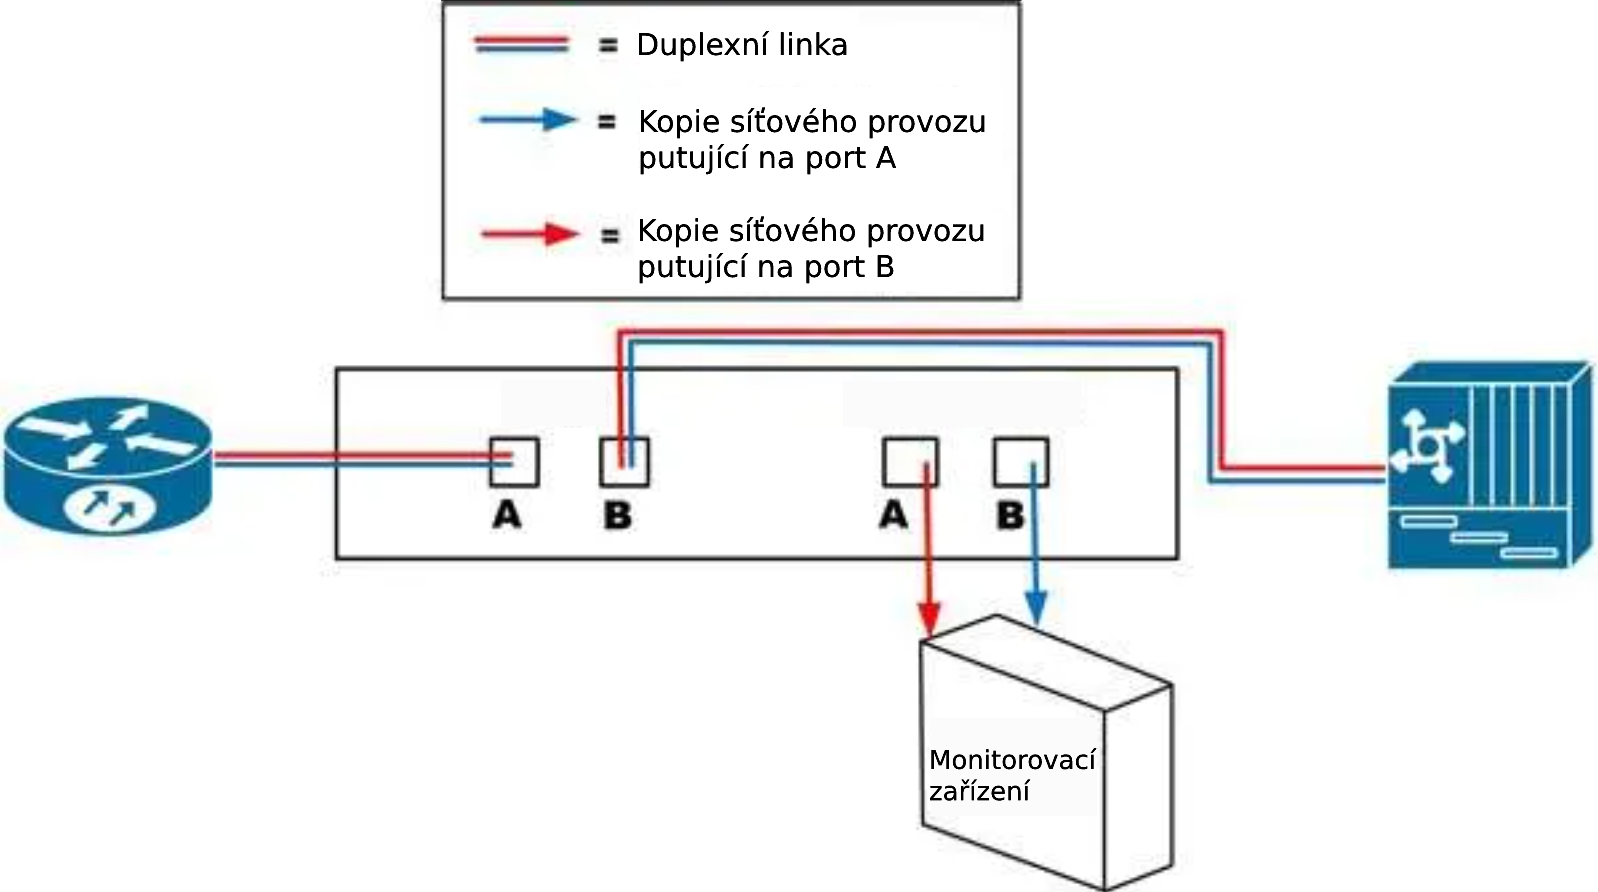
\includegraphics[scale=0.4]{obrazky-figures/ForenzniAnalyza/DukazniMaterial/inlineNetworkTap.png}
                    \caption{Demonstrace použití odposlouchávacího zařízení \textit{"inline network tap"} na drátovém komunikačním médiu mezi dvěma koncovými zařízeními.}
                    \label{fig:InlineNetworkTap}
                \end{figure}

                \item \textbf{"Upíří kohouty"} --- neboli \textit{"Vampire taps"} jsou zařízení, které na rozdíl od předešlého zařízení nevyžadují přerušení spojení a přetnutí komunikačního média. Reálné zařízení vizualizuje obrázek~\ref{fig:vampireTaps}. Toto zařízení obsahuje ostré kovové cvočky, které se skrz ochranou vrstvu a vrstvu stínění dostanou přímo na komunikační médium (typicky měď). Odposlouchávací zařízení je následně připojeno a může odposlouchávat komunikaci, aniž by se komunikace přerušila. Toto zařízení zpravidla vyvádí odposlechnutý signál pomocí portu do jiného zařízení~\cite{BookTrackingHackersReference}.
                \item \textbf{Vstupy optických vláken} --- neboli \textit{"Fiber optic taps"} odposlouchávací zařízení pro optická vlákna fungují na stejném principu jako již popsané \textit{"Inline network taps"} zařízení.
            \end{itemize}

                \begin{figure}[H]
                    \centering
                    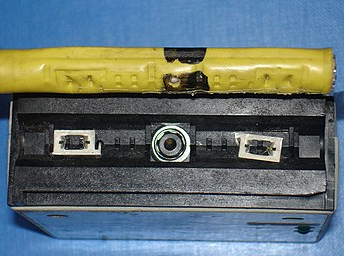
\includegraphics[scale=0.8]{obrazky-figures/ForenzniAnalyza/DukazniMaterial/vampireTap.png}
                    \caption{Ukázka použití odposlouchávacího zařízení \textit{"Vampire tap"} na drátovém komunikačním médiu. Převzato ze stránek www.wikimedia.org\footnotemark.}
                    \label{fig:vampireTaps}
                \end{figure}
                \footnotetext{Zdroj --- \url{https://upload.wikimedia.org/wikipedia/commons/thumb/7/72/VampireTap.jpg/440px-VampireTap.jpg} [5. května 2022]}
            
        \subsubsection*{Bezdrátová komunikace}
            Bezdrátová komunikace je nejčastěji zprostředkována pomocí rádiových vln, jelikož dokáží procházet skrz dřevo, cihly, sklo, tenkou vrstvu betonu, a skrz další materiály. Všechny materiály přes které vlny prochází, snižují sílu signálu. Jako komunikační médium lze použít i světlo, například infračervené avšak daleko více používané jsou rádiové vlny~\cite{ComputerNetworking}.

            Výhodou bezdrátové komunikace je, že není zapotřebí žádné drátové spojení a každý je tedy schopen komunikovat. Toto je však i nevýhodou a proto je zapotřebí, aby komunikace byla zašifrovaná. Nicméně pokud například útočník získá kryptovací klíč či prolomí šifru, má přístup k veškeré komunikaci a nikdo nezjistí, že komunikace je odposlouchávána. I přes to, že je komunikace prostřednictvím zabezpečené Wi-Fi sítě šifrována, lze z ní získat užitečné informace pro účely síťového forenzního vyšetřování~\cite{BookTrackingHackersReference}. Například lze zjistit přítomnost přístupového bodu, jeho název, \gls{MAC} adresy všech připojených zařízení a další detaily o síti.
            
        \subsubsection*{Přepínače}
            Přepínače jsou zařízení, která slouží ke směrování síťového provozu v \gls{LAN} sítích pomocí \gls{MAC} adres. Každý přepínač obsahuje \gls{CAM} neboli mapovací tabulku portů na \gls{MAC} adresy síťových karet zařízení v síti. Tuto tabulku lze použít k vyhledání konkrétního zařízení v síti. Některé přepínače také umožňují tzv. \textit{"mirror traffic", } což znamená duplikovat komunikaci z jednoho nebo více portů na jiný port, čímž je možné odposlouchávat komunikaci.~\cite{BookTrackingHackersReference}.
            
        \subsubsection*{Směrovače}
            Směrovače propojují jednotlivé podsítě a sítě a tím umožňují komunikaci v rámci různých síťových segmentů. Aby směrovač mohl směrovat pakety, musí mít směrovací tabulku, ve které se mapují porty na směrovači k jeho dostupným sítím, ke kterým má přímý přístup, ale i ke vzdáleným sítím. Směrovače si vzájemně sdílí směrovací tabulky (protokol \gls{OSPF} , \gls{RIP})~\cite{MatousekBookReference}. Směrovače dokáží filtrovat pakety dle \gls{IP} adresy či portu a tím například omezovat komunikaci. Dále také některé směrovače umí zaznamenávat komunikaci případně zamítnutých pokusů o komunikaci a posílat tyto záznamy na jiné zařízení~\cite{BookTrackingHackersReference}.
            
        \subsubsection*{\gls{DHCP} servery}
            \gls{DHCP} je mechanismus k dynamickému přidělování \gls{IP} adres. Pokud je v síti \gls{DHCP} server může v různém čase přidělit stejnou \gls{IP} adresu různý zařízením. \gls{DHCP} server si vede záznamy o přidělených adresách v čase k určitým zařízením, které identifikuje pomocí jejich \gls{MAC} adresy~\cite{ComputerNetworking}. Tyto záznamy jsou vyšetřovatelům užitečné při pátrání po fyzickém zařízení s určitou \gls{IP} adresou. Pokud je například zaznamenána neobvyklá aktivita na určité IP adrese, mohou vyšetřovatelé použít \gls{DHCP} záznamy k identifikaci fyzického zařízení, které tuto IP adresu v daném čase používalo~\cite{FundamentalsOfNetworkForensicsReference}.

        \subsubsection*{\gls{DNS} servery}
            Služba \gls{DNS} je klíčovou součástí počítačových sítích a jedním z jejích úloh je mapování doménových jmen (\url{www.vutbr.cz}) na \gls{IP} adresy (147.02.23.142). Když uživatel zadá do prohlížeče dotaz na určitou doménu, prohlížeč vytvoří dotaz na \gls{DNS} server, který odpoví s příslušnou \gls{IP} adresou. Pokud je odpověď \gls{DNS} serveru uložena v cache paměti, odpověď je vrácena okamžitě bez nutnosti kontaktovat další \gls{DNS} server. DNS servery si mohou vést záznamy o jednotlivých dotazech v čase a zaznamenávat tak aktivitu jednotlivých uživatelů. To může být zajímavou informací pro vyšetřovatele, jelikož tak mohou vědět na jaké webové stránky se uživatel dotazoval~\cite{MatousekBookReference}.
        
        \subsubsection*{Autentizační servery}
            Autentizační servery slouží k centralizované správě uživatelských účtů a autentizaci uživatelů, čímž organizace eliminuje potřebu mít v rámci jedné organizace více autentizačních systému a veškerou odpovědnost a režii s autentizací spojenou centralizuje na jedno místo. Hlavním úkolem těchto serverů je ověření totožnosti uživatele typicky uživatelským jménem a heslem, jenž se dnes zpravidla posílá šifrovanou komunikací zajištěnou protokolem SSL/TLS. Tyto servery zaznamenávají jednotlivé události jako je pokus o přihlášení. Díky těmto záznamům lze identifikovat podezřelé aktivity, jakými jsou například pokus o přihlášení z podezřelé lokace, pokus o přihlášení v podezřelou hodinu, pokusy o přihlášení hrubou silou, atd~\cite{BookTrackingHackersReference}.
            
        \subsubsection*{Webové proxy servery}
            Proxy server je komunikační prostředník mezi koncovými uzly. Ve společnostech se proxy server nejčastěji využíván k ukládání webových stránek do paměti cache a k zaznamenávání komunikace. Pokud uživatel vytvoří dotaz na webovou stránku (www.vutbr.cz), dotaz je odeslán na proxy server, který dotaz povolí, případně zamítne. Důvodem k zamítnutí může být dotaz na stránku nacházející se na černé listině pochybných webových stránek. V případě, že proxy server povolí stránku, je uživateli vrácena požadovaná odpověď~\cite{ComputerNetworking}.

            Záznam komunikace procházející přes proxy server je pro vyšetřovatele cenným zdrojem informací, jelikož tak, lze získat webovou aktivitu například všech zaměstnanců ve společnosti. Pomocí těchto záznamů, lze tak zjistit například oběť útoku zvaným \textit{"phishing"} nebo identifikovat zdroj malware viru. Pokud si proxy server ukládá webové stránky do paměti cache, je možné vidět obsah, který byl zobrazen oběti útoku~\cite{BookTrackingHackersReference}. Dalším využití proxy serverů je:
            \begin{itemize}
                \item \textbf{Ochrana soukromí} --- když klient použije proxy server, jeho \gls{IP} adresa není viditelná pro cílový server, což může chránit soukromí uživatele.
              \item \textbf{Změna geolokace} --- proxy servery umožňují překrýt geolokaci klienta a tak mu zpřístupnit obsah, který je geolokalizačně omezen.
            \end{itemize}
            
\section{Nástroje k získávání forenzních síťových dat}
Síťové forenzní nástroje jsou nezbytným nástrojem pro každého, kdo se zabývá bezpečností a správou počítačových sítí. Tyto nástroje umožňují detekovat a analyzovat útoky na síť a identifikovat bezpečnostní problémy. Síťové forenzní nástroje nám umožňují monitorovat síť a získávat informace o provozu na síti. Tyto nástroje jsou nedílnou součástí vyšetřování a pomáhají vyšetřovatelům analyzovat již spáchané útoky nebo naopak detekovat nadcházející~\cite{FundamentalsOfNetworkForensicsReference}. Některé síťové forenzní nástroje umožňují také provádět \textit{"incident response"}, což je proces rychlé reakce na bezpečnostní incidenty a minimalizace škod způsobených útokem. Vyšetření a objasnění útoku probíhá z mnoha důvodů, uvedu pouze 3 základní. 
    
    \begin{itemize}
        \item \textbf{Jak se útočník dostal do systému?} --- toto je velice důležitá otázka pokud dojde k útoku. Pokud útočník nějakým způsobem obejde zabezpečení systému je nutné zjistit jakým způsobem prolomil systémová zabezpečení a systém patřičně upravit aby nedošlo k dalšímu útoku.
        
        \item \textbf{Co útočník v systému dělal?} --- otázka, kterou si položí většina lidí a hlavně majitel onoho systému. Je důležité vědět zda došlo například k infiltraci dat ze systému ať už to jsou osobní informace zaměstnanců či jiná citlivá data. Takto infiltrovaná data mohou být zveřejněna, použita k vydírání atd.
        
        \item \textbf{Kdo je útočník?} --- zjištění pravé identity  útočníka k jeho následnému dopadení.
    \end{itemize}
    
    Tyto nástroje jsou využívány nejen vyšetřovateli pro forenzní analýzu ale také administrátory sítí k odstraňování problémů na síti, vývoji nových programů, komunikačních protokolů atd. Například mohou být použity k identifikaci slabých míst v síti, zlepšení výkonu sítě a optimalizaci použití sítě. V neposlední řadě, některé z nich jsou používány také studenty ke studijním  účelům~\cite{EnisaReference}. Síťové forenzní nástroje umožňují také vytvořit detailní logy síťového provozu, což může být užitečné pro další analýzu a zpracování dat. Tyto logy mohou být také použity k vytvoření zpráv pro management nebo jako důkazy v soudních procesech. 

    Níže uvedené nástroje jsem analyzoval z hlediska UX a UI. Cílem této analýzy bylo zjistit jak jsou nástroje implementovány. Získané znalosti jsem poté využil při návrhu mé aplikace, která je hlavním předmětem této práce. Analýzu některých nástrojů jsem prováděl přímo v aplikaci, zatímco jiné jsem analyzoval pouze na základě snímků nebo videí.    

    \subsection{Síťové forenzní nástroje pro analyzování}
    \label{forensicTools}
        Síťové forenzní nástroje pro analyzování (\gls{NFAT}) slouží zejména k analyzování a ukládání síťových dat jakožto důkazních materiálů k jejich následnému šetření. Mohou být jak softwarové tak hardwarové. Existují jak proprietární, tak i open-source nástroje. Většina open-source nástrojů je vytvořena pro prostředí Linux. Jelikož se jedná o open-source licenci, lze tyto nástroje libovolně modifikovat, doprogramovávat funkcionalitu a přizpůsobit si nástroj konkrétním potřebám~\cite{FundamentalsOfNetworkForensicsReference}.
        
        Síťoví analytici a vyšetřovatelé běžně analyzují odposlechnuté pakety za účelem identifikace paketů, které mají specifický význam pro vyšetření případu. Jelikož na síti může být velký provoz, jednotlivé pakety lze filtrovat podle komunikačního protokolu, čísla portu, adresy odesílatele/příjemce, případně podle obsahu paketu a jiných kritérií k identifikování konkrétních paketů.
    
        \subsubsection*{NetDetector}
            NIKSUN NetDetector je sytém pro analyzování síťového provozu postavený na NIKSUN architektuře. Poskytuje zachycování paketů, generování metadat, \gls{IDS}/\gls{IPS} systémy, rekonstrukci jednotlivých relací a jiné~\cite{NiksunNetDetectorReference}. Díky těmto funkcím může NIKSUN NetDetector poskytnout uživatelům velmi podrobné informace o provozu v jejich sítích. Niksun NetDetector má dvě varianty:
            \begin{itemize}
                \item NetDetector --- desktopová aplikace poskytuje uživatelům vysokou rychlost a efektivitu při analýze síťového provozu. 
                \item NetDetector Live --- webová aplikace je pak ideální pro uživatele, kteří potřebují přístup k systému z různých zařízení a míst.
            \end{itemize}
            
            NetDetector je využíván více než tisíci společnostmi včetně společností Fortune 500, vládních agentur a internetových providerů~\cite{NiksunNetDetectorIBMReference}. Díky této popularitě se jedná o osvědčený a spolehlivý nástroj pro analýzu síťového provozu.
    
        \subsubsection*{Xplico}
            Xplico je open-source nástroj pro forenzní analýzu paketů na UNIX systémech. Podporuje celou řadu protokolů, včetně \gls{HTTP}, \gls{SIP}, \gls{IMAP}, \gls{POP}, \gls{SMTP}, \gls{TCP}, \gls{UDP}, IPv6, Facebook, \gls{MSN}, \gls{RTP}, \gls{IRC}, Paltalk, a dalších.
            Cílem aplikace Xplico je extrahovat aplikační data ze zachyceného provozu~\cite{XplicoReference}. Detailní popis tohoto nástroje naleznete v kapitole~\ref{sec:XplicoNetworkMiner}.
                   
        \subsubsection*{NetworkMiner}
            Dalším velice populárním nástrojem pro odposlech a analýzu je NetworkMiner, který má taktéž open-source licenci, avšak lze zakoupit i profesionální licence s rozšířenou funkcionalitou např. export \gls{XML}, extrakce audio hovorů atd. Byl vyvinut v roce 2007 a od té doby se stal velice populárním nástrojem používaným společnostmi po celém světě. Primárně byl vyvinut pro operační systém Windows, ale lze jej použít i na systému Linux a MacOS. Detailní popis tohoto nástroje naleznete v kapitole~\ref{sec:XplicoNetworkMiner}.

    \subsection{Síťové programy pro skenování}
            Existuje celá řada nástrojů pro síťové skenování, které mají různé funkce a vlastnosti. V této sekci uvedu Angry \gls{IP} Scanner a Wireless Network Watcher. Síťové skenování může být užitečné pro správce sítě, kteří potřebují získat přehled o aktivních zařízeních a službách v síti. Vyhledávání probíhá za pomocí \textit{"ping sweepování"}, které vrací informace o aktivních uživatelích v síti a port jejich nabízené služby. Je možné invertovat tento proces za účelem vyhledání, která \gls{IP} adresa patří aktivnímu uživateli~\cite{FundamentalsOfNetworkForensicsReference}. 
            
            \subsubsection*{Angry \gls{IP} Scanner}
                Angry \gls{IP} Scanner, taktéž zvaný IPScan je multiplatformní nástroj s open-source licencí s více než 29 miliony stažení i přestože instalace není nutná. Angry \gls{IP} Scanner lze používat přímo v prohlížeči a jedinou prerekvizitou je Java Runtime Environment. IPScan dokáže skenovat \gls{IP} adresy a jejich porty jakékoliv vzdálenosti. Naskenované výsledky lze uložit do \textit{.csv}, \textit{.txt}, \textit{.xml} souborů. Angry \gls{IP} Scanner skenuje síť více vláknovým přístupem za účelem zvýšení rychlosti skenování~\cite{IPScanReference}.

            \subsubsection*{Wireless Network Watcher}
                Wireless Network Watcher je \textit{"freeware"} nástroj vyvinutý společností NirSoft Inc. Skenuje bezdrátové sítě a pro každý aktivní uzel zajistí \gls{IP} adresu, \gls{MAC} adresu, NIC\footnote{Network interface controller - síťová karta, která připojuje zařízení k počítačové síti} výrobce, název zařízení, datum prvního spuštění a status~\cite{FundamentalsOfNetworkForensicsReference}. Podporuje exportování vyhledaných výsledku do \textit{.xml}, \textit{.txt}, \textit{.html} a dalších souborů.
                
        \subsection{Síťové nástroje pro monitorování}
            Nástroje pro monitorování sítě konstantně monitorují síť a upozorní na anomálii  administrátora pokud se síť vyskytne v předem definovaném stavu~\cite{EnisaReference}. Typickým stavem pro vytvoření upozornění, je například nedostupnost nějaké služby, způsobená pádem serveru. Síťové monitorování je v podstatě kolekce jednoduchých nástrojů a příkazů operačního systému. Typicky se při monitorování sleduje výkonost, \gls{QOS}, doba odezvy, šířka pásma, atd~\cite{FundamentalsOfNetworkForensicsReference}.

            \subsubsection*{Wireshark}
            Jedním z nejznámějších a nejpoužívanějších síťových nástrojů pro odposlech a analýzu paketů je právě Wireshark, původně pojmenovaný Ethereal. Wireshark je open-source dostupný na GNU/Linux, Windows, MacOS a ostatních UNIX systémech. Pro odposlech paketů Wireshark používá libpcap\footnote{Multiplatformní knihovna, poskytující aplikační rozhraní k příjímání paketů ze sítě~\cite{LibpcapReference}} pro odposlechnutí paketů ze sítě. Sítě, které nepodporují libpcap, Wireshark nedokáže odposlouchávat~\cite{FundamentalsOfNetworkForensicsReference}. 
            
            Wireshark analyzuje pakety pomocí nástroje tshark, který je součástí Wiresharku. Pomocí nástroje Wireshark lze také analyzovat předem odposlechnutou komunikaci uloženou ve formátu \textit{.pcap} a poskytnout základní informace o paketech. Poskytuje jak uživatelsky přívětivé grafické prostředí, tak i ovládání pomocí příkazové řádky. Wireshark nabízí filtrování irelevantních paketů dle uživatelských preferencích. Existuje více než 105000 různých kombinací filtrů, které může uživatel zvolit a tím zpřesnit zobrazení paketů, které uživatele zajímají. 
            
            Nástroj Wireshark také využívá Ngrep\footnote{Nástroj postavený nad knihovnou libpcap k identifikování paketů obsahující či neobsahující vyhledávaný řetězec či binární sekvenci kdekoliv v paketu~\cite{BookTrackingHackersReference}} avšak tento nástroj prohledává vyhledávaný obsah v každém paketu zvlášť. Což znamená, že pokud je právě vyhledávaný obsah rozprostřen do více paketů, tak jej Ngrep nenajde~\cite{BookTrackingHackersReference}.

            \begin{figure}[H]
                \centering
                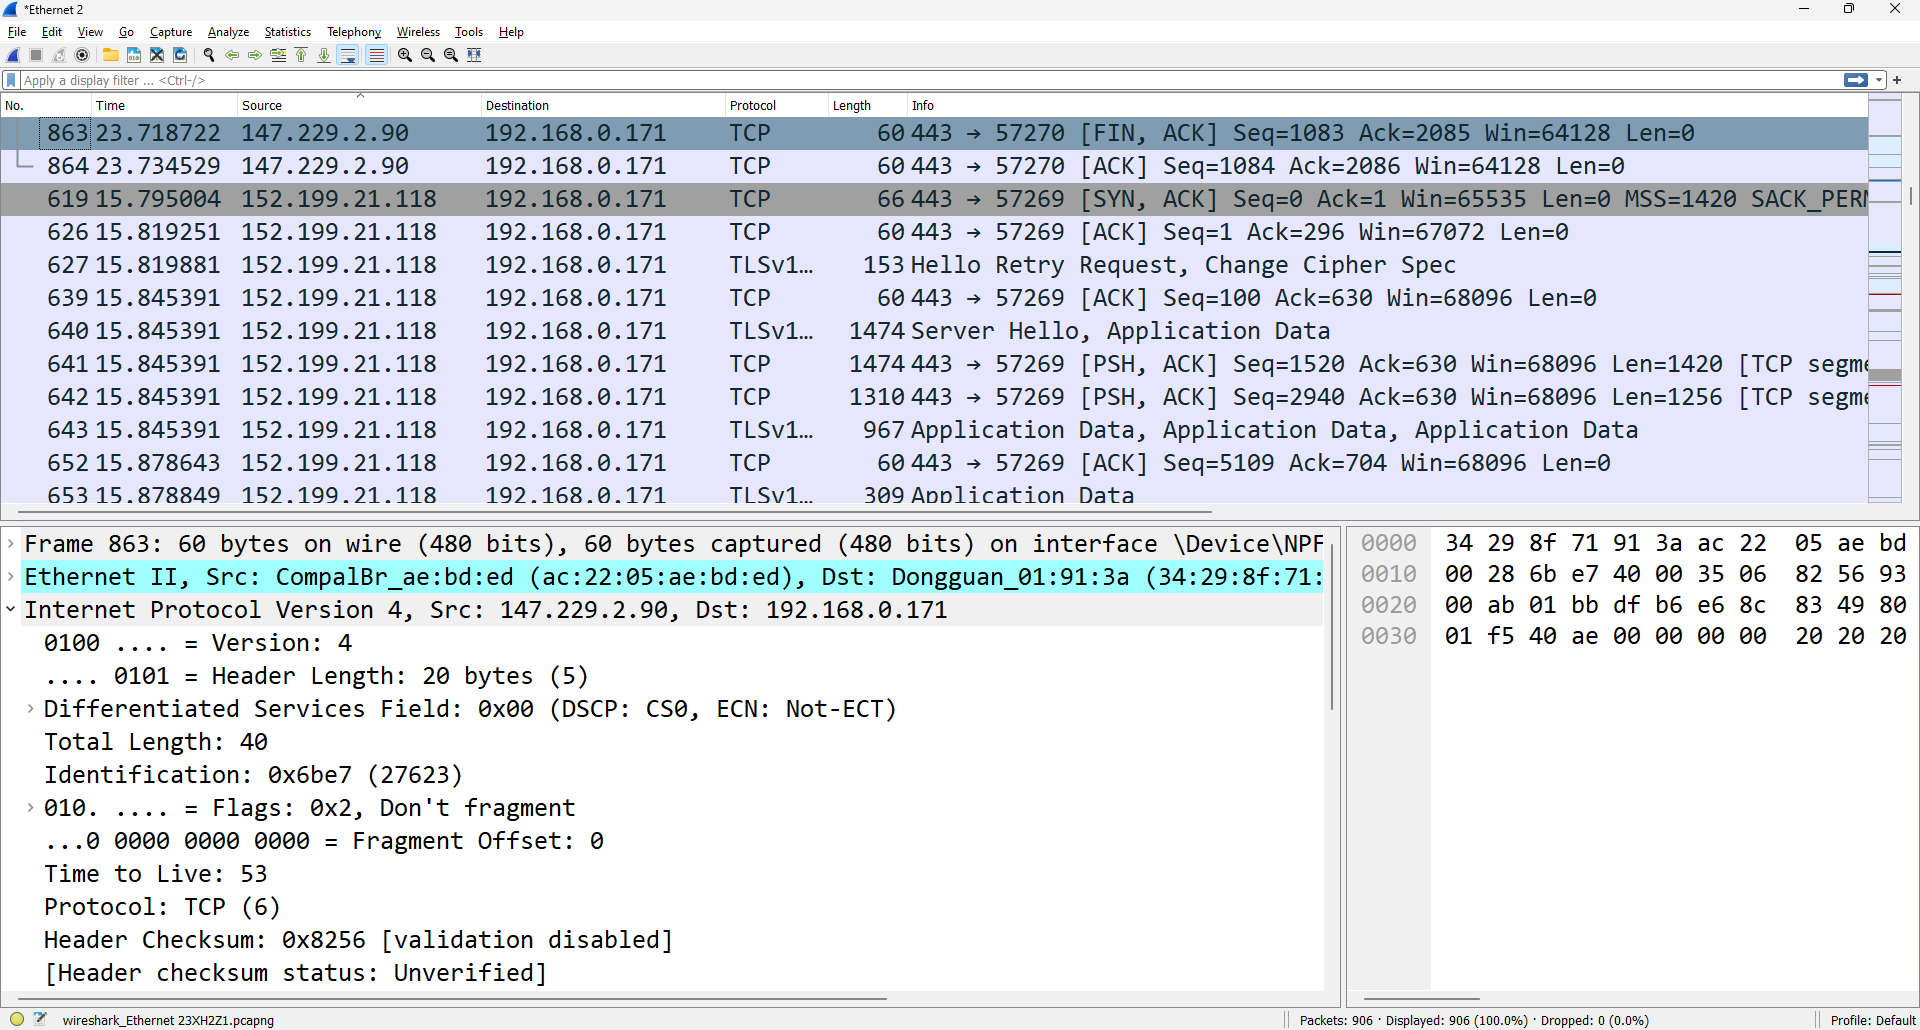
\includegraphics[scale=0.35]{obrazky-figures/ForenzniAnalyza/tools/Wireshark.png}
                \caption{Ukázka zachycené komunikace v programu Wireshark.}
                \label{fig:my_label}
            \end{figure}          
                
            \subsubsection*{VisualRoute}
                VisualRoute je diagnostický nástroj, dostupný na Windows a MacOS systémy, který vizuálně zobrazuje výsledky \textit{"traceroute"} programu. Mezi klíčové nástroje tohoto programu patří nepřetržité trasování, reverzní trasování, skenování sítě, grafické znázornění doby odezvy atd.
                
            \subsubsection*{Ntop}
                Ntop je open-source nástroj, který lze používat jak ve webovém prohlížeči tak pomocí příkazové řádky. Při použití webového prostředí Ntop vykresluje grafy a poskytuje statistické hodnoty z výsledků. Nástroj Ntop umí analyzovat komunikační provoz na síti, filtrovat výsledky a geolokalizovat hosty~\cite{FundamentalsOfNetworkForensicsReference}.
            
    
        \subsection{Nástroje pro posouzení zranitelnosti systému}
            V dnešní době, kdy jsou informační systémy často napadány a zneužívány neoprávněnými osobami, je důležité mít k dispozici nástroje, jenž posoudí zranitelnost těchto systémů. Mezi jedny ze známějších patří Metasploit a Nessus. Tyto nástroje skenují systém a hledají známé systémové bezpečnostní problémy. V některých případech mohou připomínat útok na systém za účelem vyhledání bezpečnostních děr v systému.

            \subsubsection*{Metasploit}
                Metasploit je nástroj pro testování průniknosti systémů, dostupný na Windows, Linux a MacOS. Na operačním systému Kali Linux je Metasploit předinstalovaný. Přichází ve dvou verzích Metasploit Framework (open-source) a Metasploit Pro (komerční). 
                \begin{itemize}
                    \item \textbf{Metasploit Framework} --- platforma poskytující psaní, testování a spouštění tzv. exploit programů. Obsahuje nástroje, se kterými lze testovat bezpečnostní zranitelnosti, provádět útoky atd. MSFconsole poskytuje rozhraní pro práci s Metasploit frameworkem~\cite{MetaspoiltFrameworkReference}.

                    \item \textbf{Metasploit Pro} --- na rozdíl od Metasploit Frameworku, Metasploit Pro přichází s webovým rozhraním. Dále také nabízí exploit programy, průvodce standardními audity, testování webových aplikací proti top 10 \gls{OWASP} bezpečnostních pochybností a další funkcionality~\cite{MetaspoiltProReference}. 
                \end{itemize}

            \subsubsection*{Nessus}
                Nessus vlastněný společností Tenable Network Security je nástroj dostupný na Windows, Linux, Solaris, FreeBSD a MacOS. Přichází ve dvou variantách Nessus Expert a Nessus Professional a obě tyto verze jsou komerční. Nessus disponuje nejnižším počtem falešně pozitivních výsledků (0.32 zmetků při milionů skenování) a má nejširší pokrytí ze všech nástrojů v tomto odvětví~\cite{NessusReference}.
        

\section{Analýza nástrojů Xplico a NetworkMiner}
\label{sec:XplicoNetworkMiner}

    Nástroje Xplico a NetworkMiner byly již stručně popsány v předešlé kapitole~\ref{forensicTools}. V této kapitole se budu zabývat analýzou těchto forenzních nástrojů detailněji. Pokusím se uvést silné a slabé stránky těchto nástrojů a na závěr každého z nástrojů uvedu případy užití, které slouží k demonstraci jejich funkcionality. 

    NetworkMiner a Xplico patří mezi předně používané nástroje a oba disponují open-source licencí. Nástroje slouží k analyzování a následné vizualizaci forenzně síťových dat. Jsou navrženy tak, aby usnadňovali práci vyšetřovatelům a odborníkům v oboru informační bezpečnosti. Usnadnění práce následně vede k významnému urychlení řešených případů, což může vést ke snížení kybernetických útoků. Oba tyto nástroje lze také využít ke studijním účelům nebo pro monitorování a diagnostiku síťových problémů. Získané poznatky z těchto nástrojů budou aplikovány při tvorbě nástroje pro vizualizaci forenzně síťových dat, který je hlavním záměrem této práce. 

    
    \subsection{Xplico}
        Síťový forenzní nástroj pro analýzu Xplico je nástroj vyvinutý pouze pro operační systém Linux a k zobrazení analyzovaných dat a interakci s uživatelem používá webové rozhraní. Xplico provádí analýzu dat nad již zachycenými daty, které lze nahrát v souboru s formátem patřícím do rodiny formátů \textit{.pcap} a zároveň lze pomocí tohoto nástroje zachytávat síťovou komunikaci v reálném čase. Analyzování a odchytávání paketů se provádí nad knihovnou libpcap. Xplico podporuje mnoho protokolů (vypsány v kapitole~\ref{forensicTools}).
        
        Xplico podporuje přístup k jednomu případu více uživatelům, což může být vhodné například pro vyšetřovatele, pracující na stejném případu. Lze využít databázi SQLite, MySQL či PostgreSQL pro zachování persistence dat~\cite{XplicoReference}. Dále umožňuje filtrovat a procházet zachycená data podle jistých kritérií, jako jsou například čísla portů, použitý protokol a jiné. Analyzovaná data je možné exportovat do formátu \textit{.xml} a používat dále v jiných nástrojích.

        Xplico poskytuje dokumentaci popisující jak nástroj nainstalovat a základní použití, avšak u komerčních nástrojů bývá dokumentace rozsáhlejší. Grafické prostředí není zcela uživatelsky přívětivé, na některých stránkách chybí popis zobrazených dat a uživatel tak neví, co zobrazená data znamenají\footnote{Například při zobrazení detailní stránky zachyceného emailu, Xplico zobrazí dvě emailové adresy a není u nich popis, kdo je odesílatel a kdo adresát.}. Dalším velkým nedostatkem je chybějící agregace dat dle nějakého kritéria nebo agregace kolekce zachycených zpráv v podobě grafů. V následující části této kapitoly předvedu jeden běžný případ užití popisující základní funkcionalitu nástroje Xplico a jeden specifický soutěžní, který popisuje práci s nástrojem Xplico při řešení konkrétního případu.
        
        \subsubsection*{Běžný případ užití}
            Následující diagram užití slouží k vizuální reprezentaci různých scénářů, které lze provádět s tímto nástrojem. Tento diagram zahrnuje všechny funkcionality nástroje Xplico. Diagram je zde zobrazen k porovnání funkcionalit s nástroji NetworkMiner a mnou vytvořené Blazor aplikace.
                \begin{figure}[H]
                    \centering
                    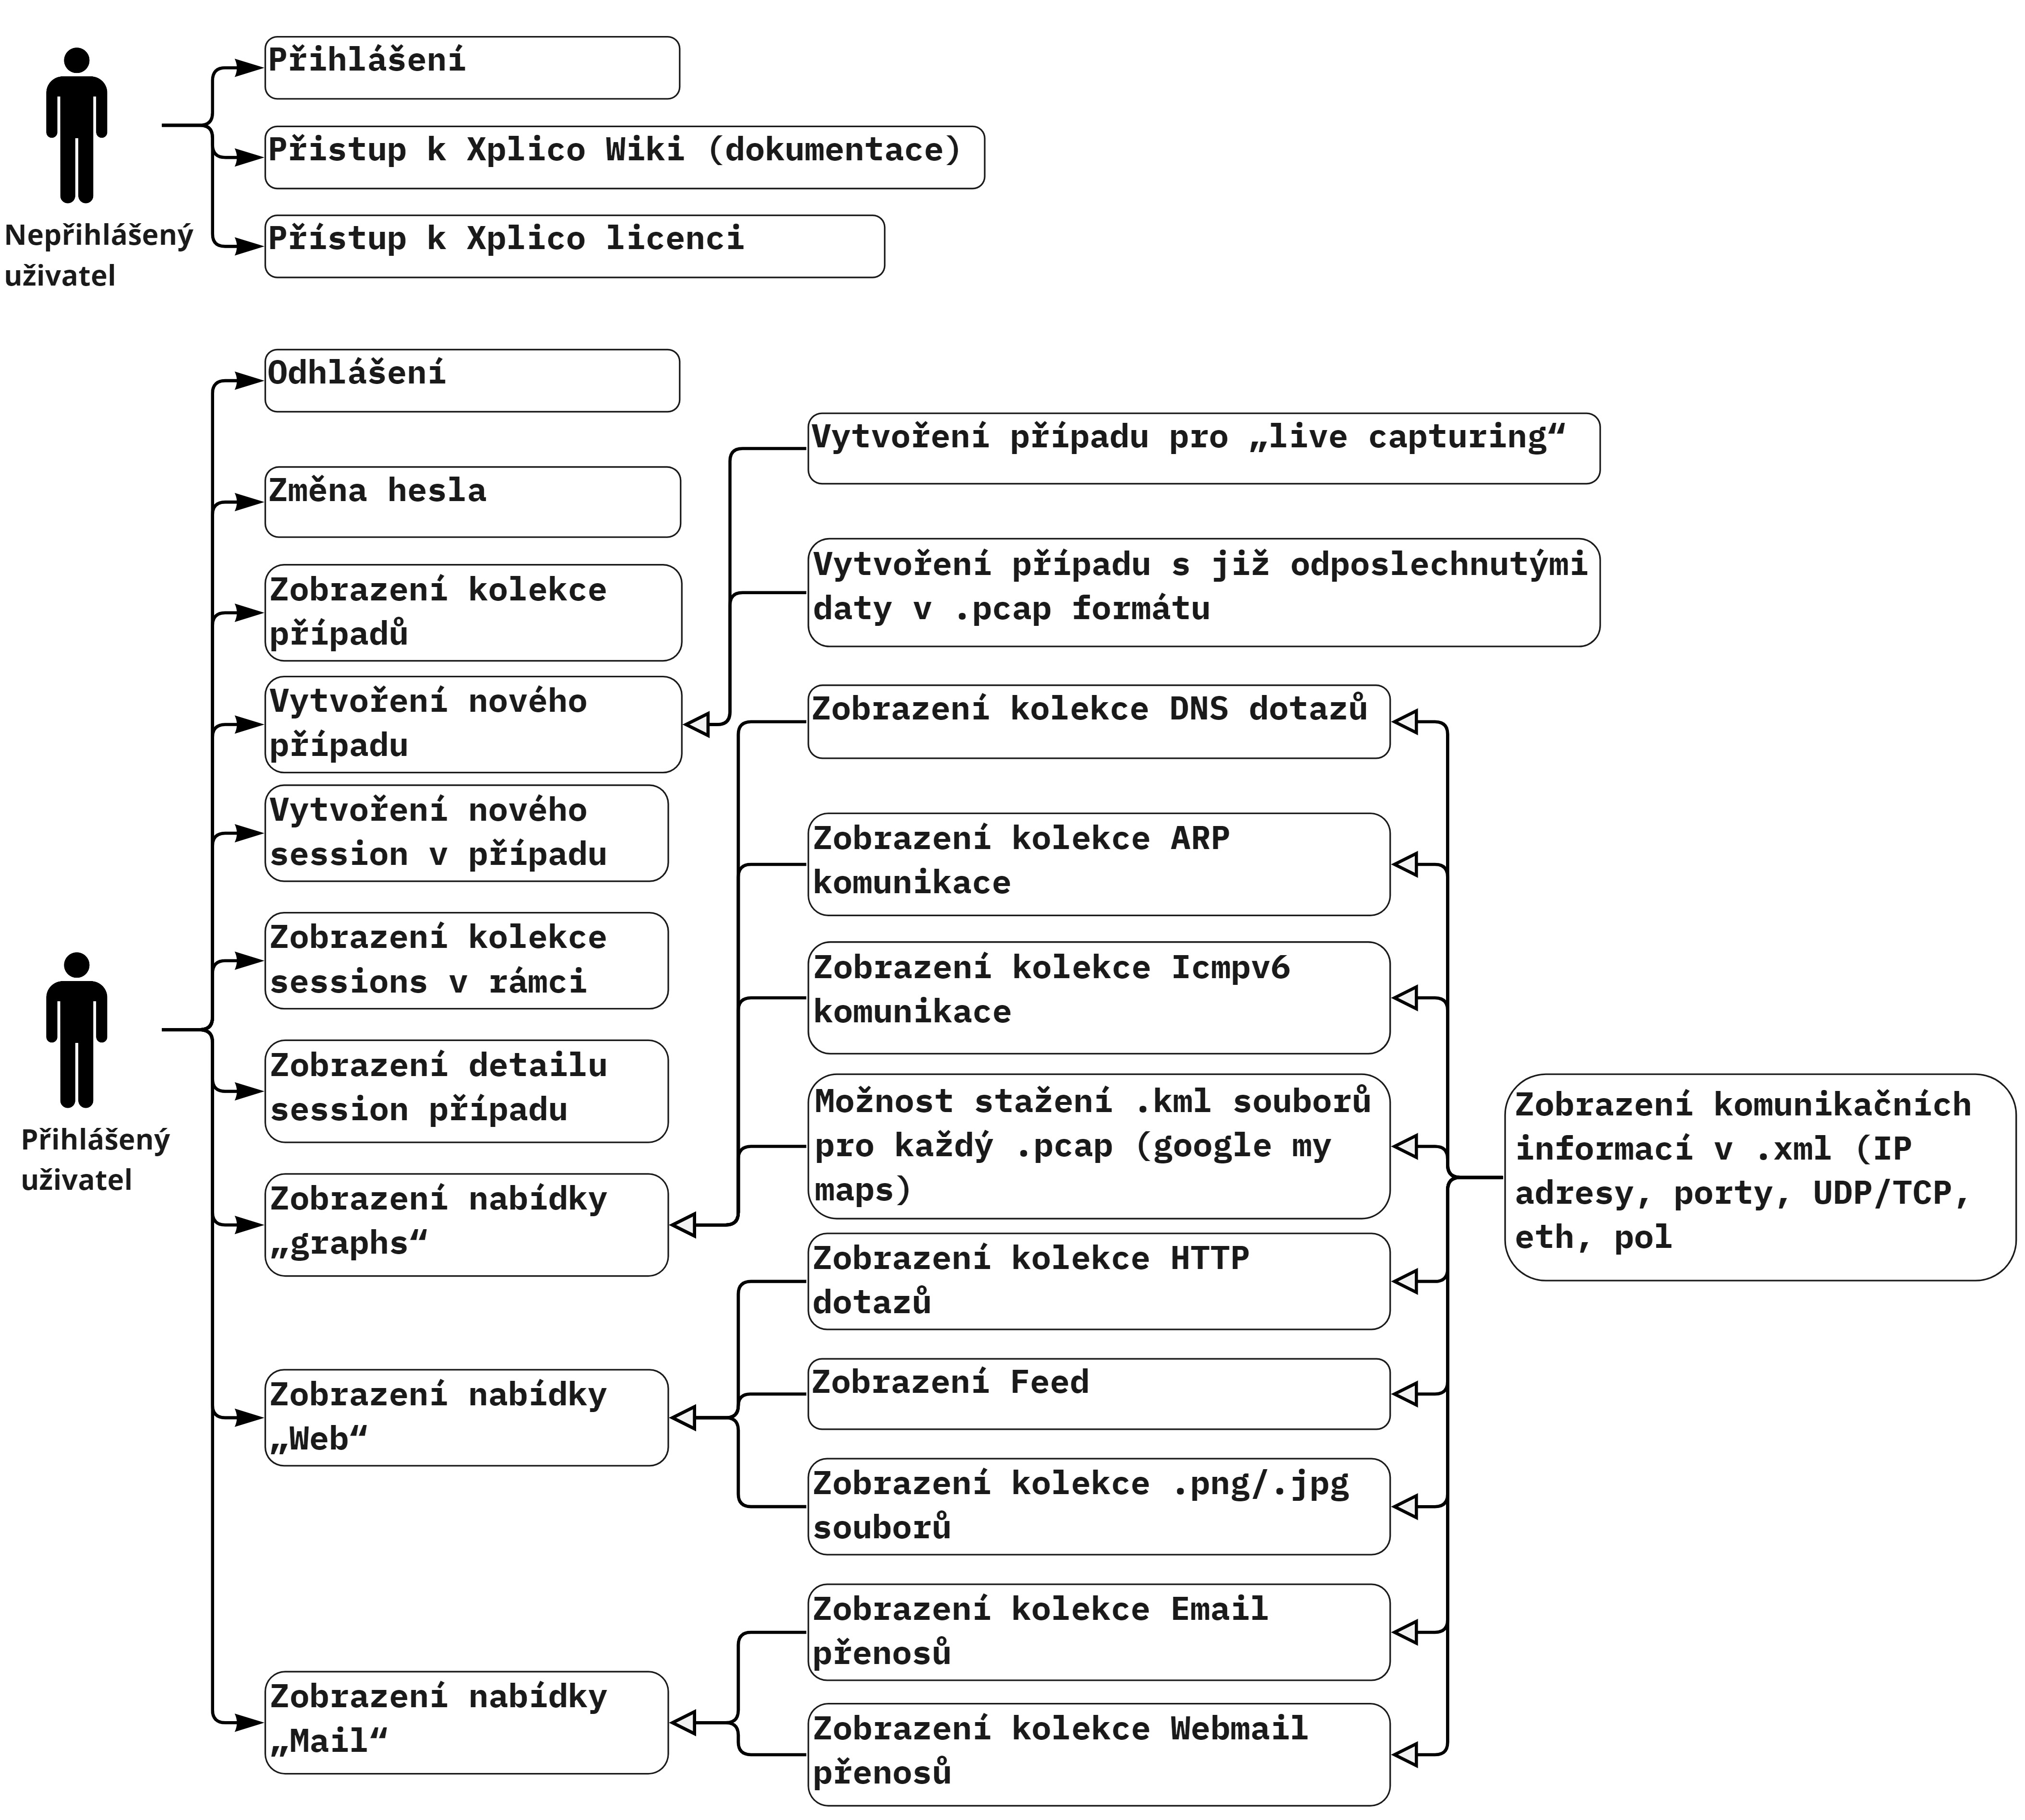
\includegraphics[scale=0.1]{obrazky-figures/usecases/Xplico_usecase1.jpg}
                    \caption{První část případu užití síťového forenzní nástroje pro analyzování Xplico.}
                    \label{fig:my_label}
                \end{figure}
                \begin{figure}[H]
                    \centering
                    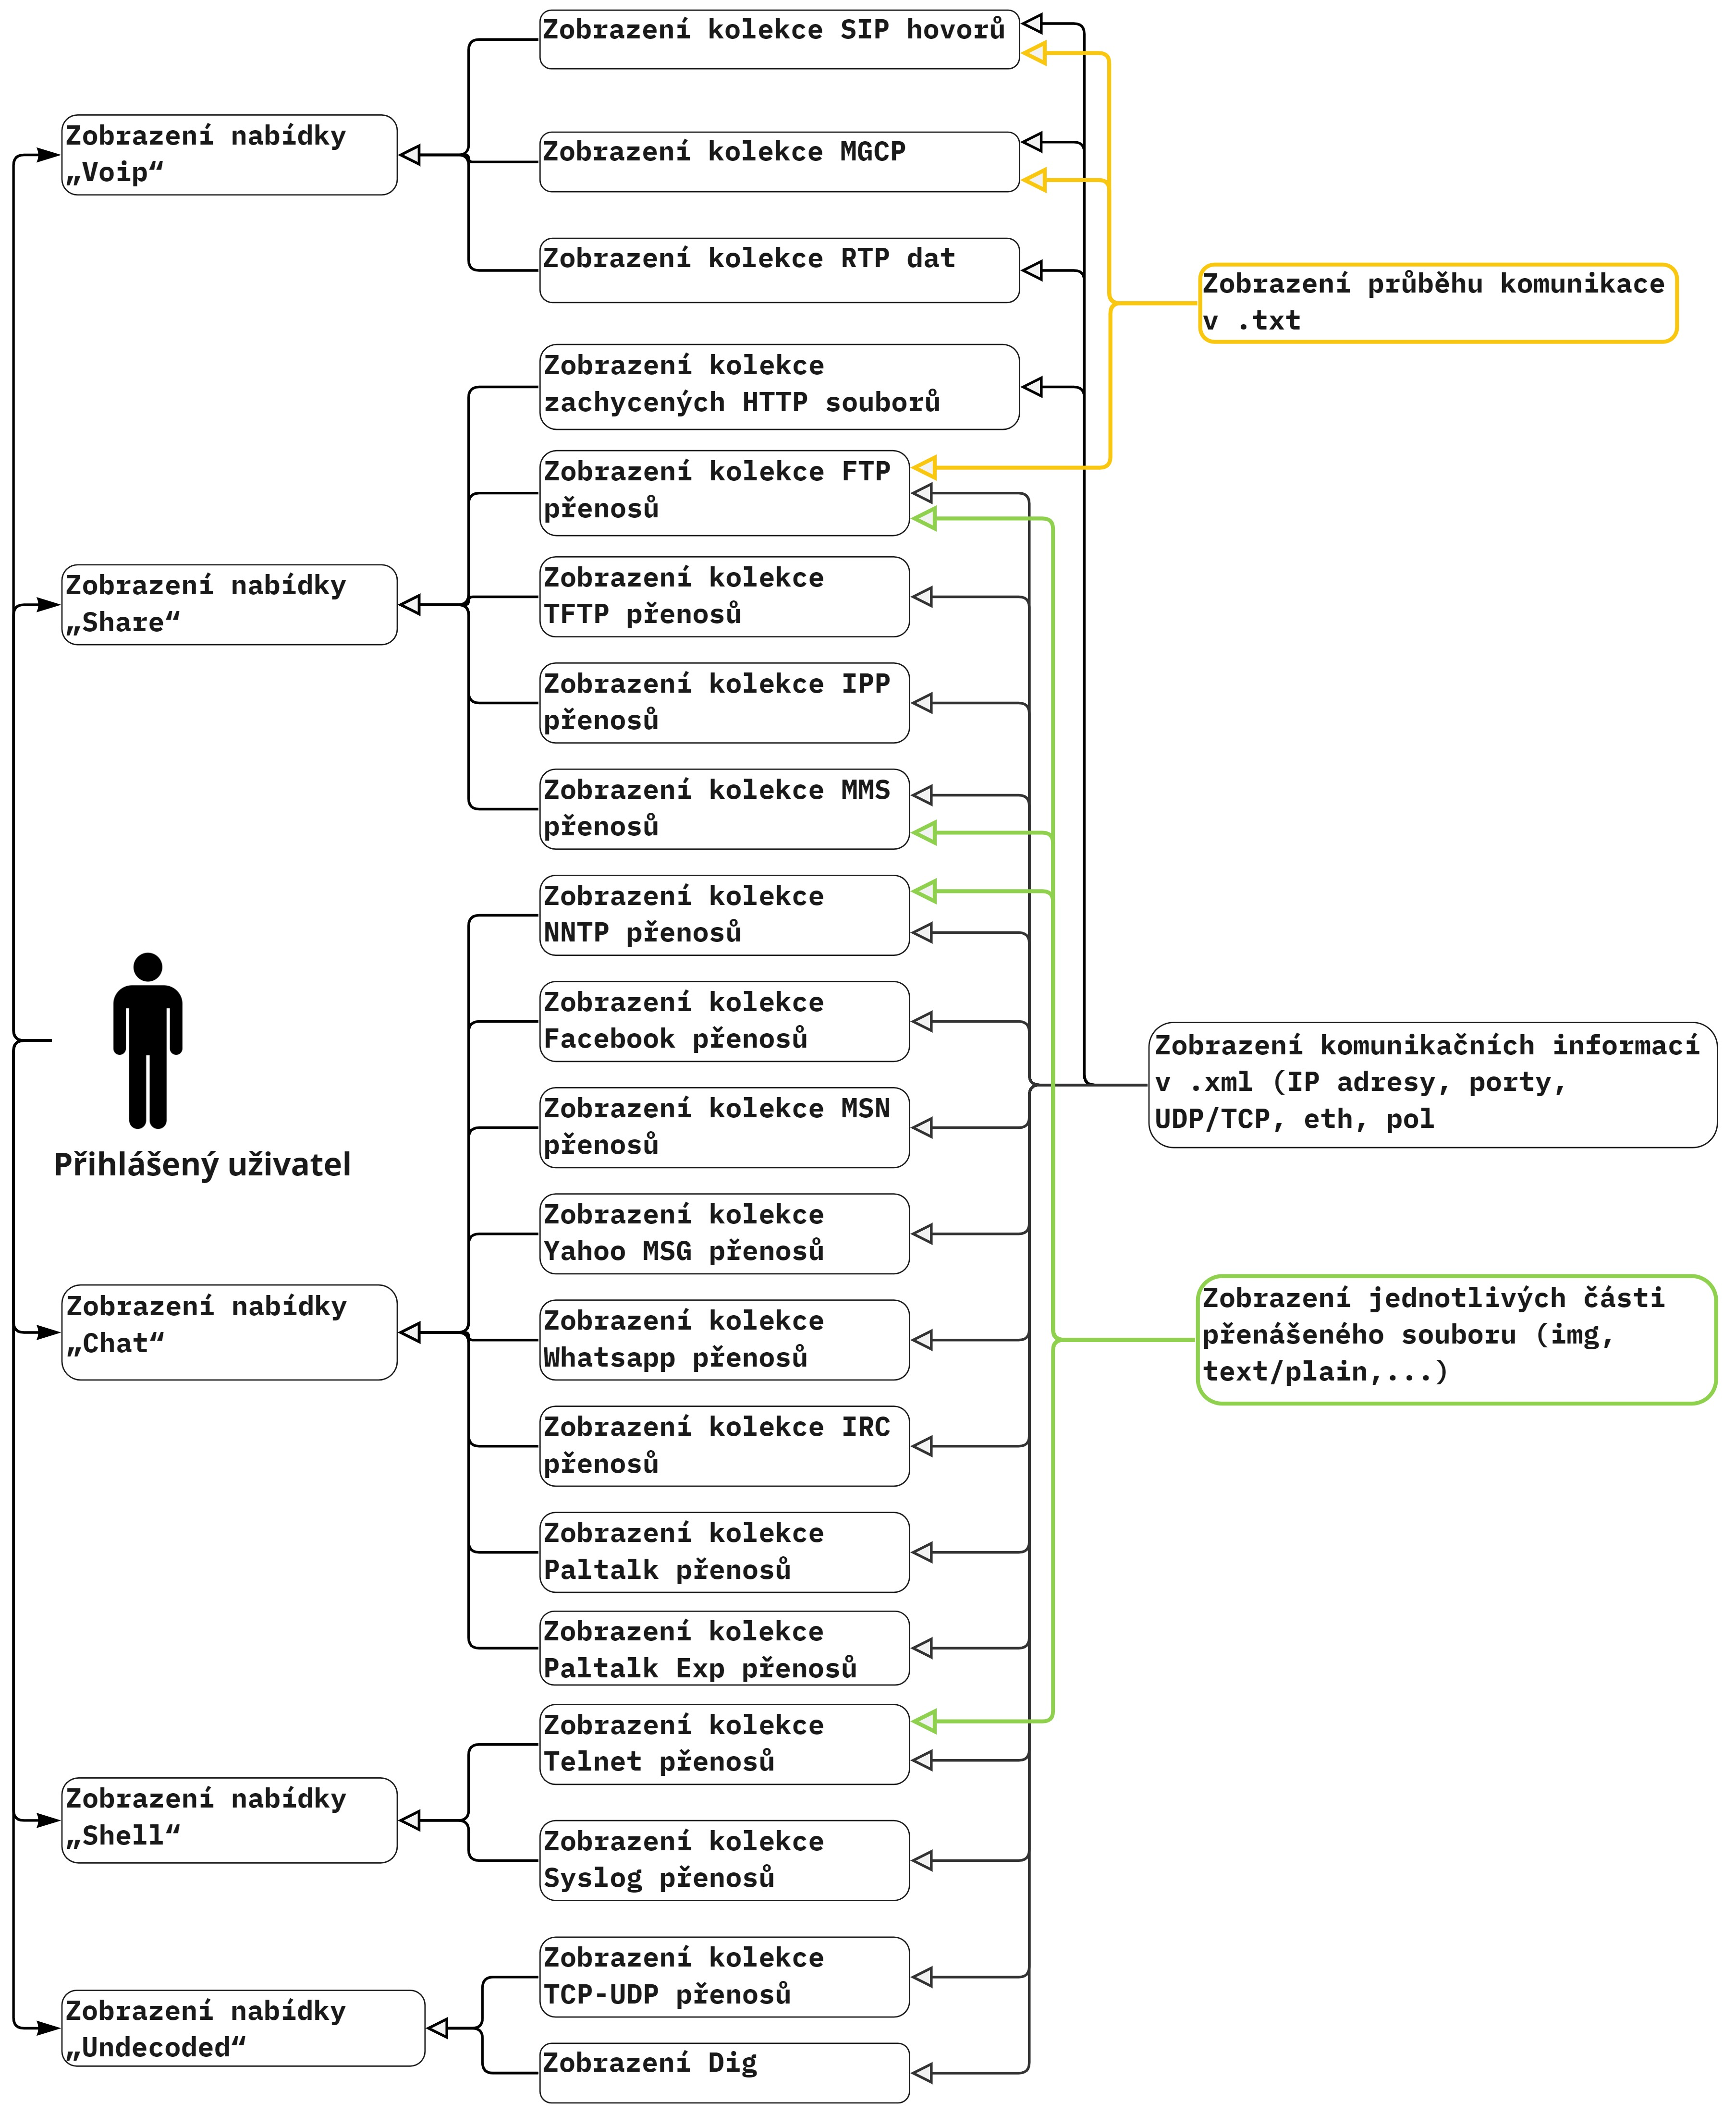
\includegraphics[scale=0.13]{obrazky-figures/usecases/Xplico_usecase2.jpg}
                    \caption{Druhá část případu užití síťového forenzní nástroje pro analyzování Xplico.}
                    \label{fig:my_label}
                \end{figure}
            \subsubsection*{Specifický případ užití nástroje Xplico}
            \label{specUseCaseXplico}
                Při vytváření úloh pro tento případ užití jsem se inspiroval soutěžním\footnote{https://forensicscontest.com/2009/10/10/puzzle-2-ann-skips-bail --- Kompletní zadání včetně odkazu ke stažení zachycené komunikace. Citováno dne 7. 2. 2023.} zadání specifických incidentů společně se zachycenou komunikací. V nástroji Xplico jsem prováděl jednotlivé úlohy a popsal jak získat pomocí tohoto nástroje hledaná data, to zobrazuje tabulka~\ref{tab:XplicoSpecialUseCase}. Cílem přpadu užití je zjistit informace o jisté Anně a jejím milencem z elektronické pošty.

\begin{center}
\begin{table}[ht]
    \centering
    \def\arraystretch{1.5}
    \begin{tabular}{| p{0.02\linewidth} | p{0.93\linewidth} |}
    \hline
        \textbf{1}   & \textbf{Jaká emailová adresa náleží Anně?} \\ \hline
            & Zobrazení kolekce emailů v záložce "\textit{Mail}". Po otevření detailu emailové zprávy lze u emailového jména "\textit{sneakyg33k@aol.com}" vidět jméno Anny. \\ \hline
            
        \textbf{2}   & \textbf{Jaká je emailová adresa milence Anny?} \\ \hline
            & Zobrazením kolekce emailů v záložce \textit{"Mail"} a analyzováním jednotlivých zpráv zaslaných Annou lze určit adresáta. \\ \hline

        \textbf{3}   & \textbf{Jaké dva předměty řekla Anna svému milenci aby přinesl?} \\ \hline
            & Zobrazení kolekce emailů v záložce \textit{"Mail"}. Vyhledání zprávy pro adresáta \textit{"mistersecretx@aol.com"} a otevření detailu zprávy. \\ \hline

        \textbf{5}   & \textbf{ Kolik příloh odeslala Anna celkem?} \\ \hline
            & Xplico nezobrazuje celkový počet příloh konkrétního odesílatele. Je tedy nutné otevřít každou elektronickou zprávu a manuálně je spočítat. \\ \hline
            
        \textbf{4}   & \textbf{Název přílohy, kterou Anna poslala svému milenci?} \\ \hline
            & Zobrazení kolekce emailů v záložce \textit{"Mail"}. Vyhledání zprávy pro adresáta \textit{"mistersecretx@aol.com"}. Po otevření detailu zprávy lze vidět jednotlivé přílohy připojené ke zprávě. \\ \hline

    \end{tabular}
    \caption{Specifický případ užití nástroje Xplico.}
    \label{tab:XplicoSpecialUseCase}
\end{table}
\end{center}
                    
    \subsection{NetworkMiner}   
        Síťový forenzní nástroj pro analýzu NetworkMiner je multiplatformní nástroj, který přichází ve dvou variantách a těmi jsou \textit{"NetworkMiner Free Edition"}, která má open-source licenci a \textit{"NetworkMiner Professional"}. Verze NetworkMiner Professional je placenou verzí, která nabízí přidanou funkcionalitu (export do \textit{.xml}, \textit{.csv}, geolokalizaci IP adresy, extrahování audio záznamu VoIP hovorů a další).

        NetworkMiner poskytuje jak analýzu již zachycené komunikace, tak aktivní odposlech síťové komunikace ze síťového rozhraní. Lze jej také použít pro extrahování souborů, emailů a hesel ze zachycené komunikace v souborech \textit{.pcap}~\cite{NetworkMinerReference}. NetworkMiner shromažďuje data spíše o uživateli než data o provozu na síti tzn. \gls{IP} adresu, hostname, operační systém, porty, přihlašovací údaje zadané uživatelem, atd~\cite{FundamentalsOfNetworkForensicsReference}. Přestože je NetworkMiner velice intuitivní aplikací, chybějící dokumentace tohoto nástroje může být pro některé uživatele problémem. Dalším velkým nedostatkem je chybějící agregace dat dle nějakého kritéria nebo agregace kolekce zachycených zpráv v podobě grafů. V následující části této kapitoly předvedu jeden běžný případ užití popisující základní funkcionalitu nástroje NetworkMiner a jeden specifický soutěžní, který popisuje práci s nástrojem NetworkMiner při řešení konkrétního případu.
       
        \subsubsection*{Běžný případ užití}
            Následující diagram užití slouží k vizuální reprezentaci různých scénářů, které lze provádět s tímto nástrojem. Tento diagram zahrnuje všechny funkcionality nástroje NetworkMiner. Diagram je zde zobrazen k porovnání funkcionalit s nástroji Xplico a mnou vytvořené Blazor aplikace.
            \begin{figure}[H]
                \centering
                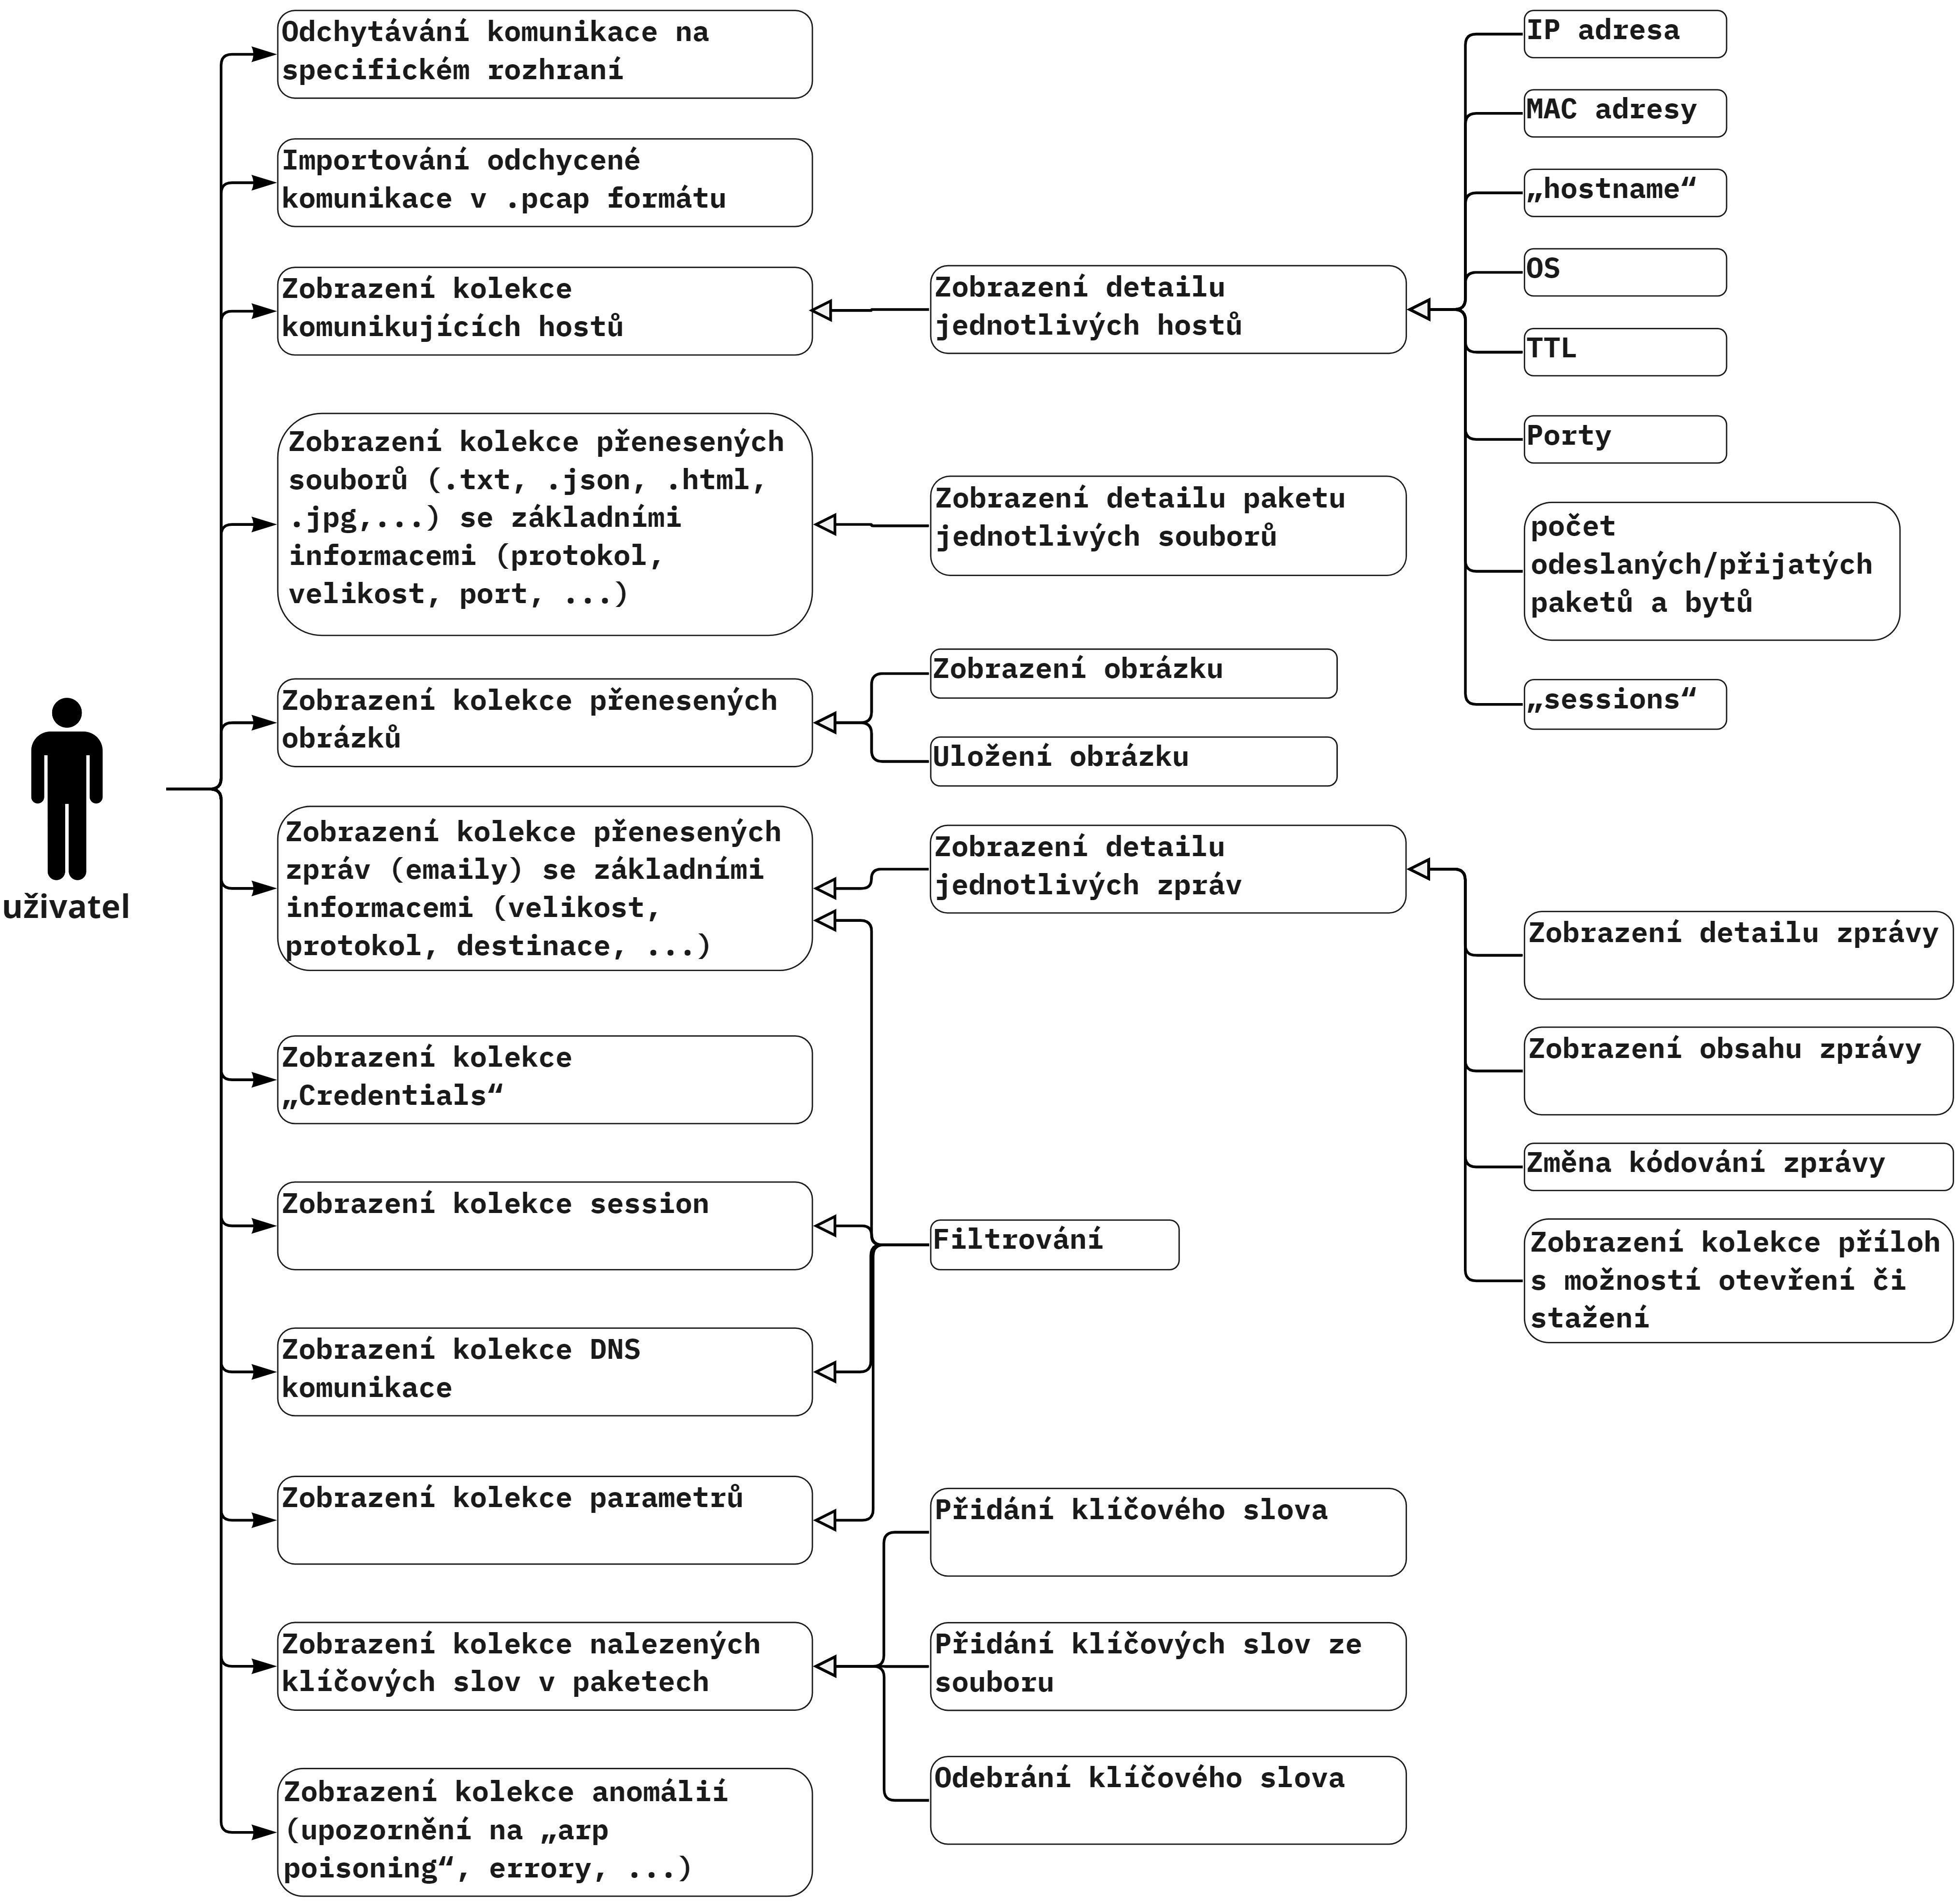
\includegraphics[scale=0.1]{obrazky-figures/usecases/NetworkMiner_usecase.jpg}
                \caption{Případ užití síťového forenzní nástroje pro analyzování NetworkMiner.}
                \label{fig:my_label}
            \end{figure}
        \subsubsection*{Specifický případ užití}
            Pro tento případ užití jsem využil stejné úlohy jako při analyzování nástroje Xplico viz sekce~\ref{specUseCaseXplico} v této kapitole. V následující tabulce~\ref{tab:NetworkMinnerSpecialUseCase} můžete vidět jak lze jednotlivé úlohy řešit pomocí nástroje NetworkMiner.
            
\begin{center}
\begin{table}[ht]
    \centering
    \def\arraystretch{1.5}
    \begin{tabular}{| p{0.02\linewidth} | p{0.93\linewidth} |}
    \hline
        \textbf{1}   & \textbf{Jaká emailová adresa náleží Anně?} \\ \hline
            & Zobrazení kolekce zpráv v záložce \textit{"Messages"}. U jména Anny lze vidět emailovou adresu a tedy odpověď: 
            \textit{"sneakyg33k@aol.com"} \\ \hline
            
        \textbf{2}   & \textbf{Jaká je emailová adresa milence Anny?} \\ \hline
            & Zobrazení kolekce emailů v záložce \textit{„Mail“}. Analyzováním jednotlivých zpráv zaslaných Annou lze určit adresáta. \\ \hline

        \textbf{3}   & \textbf{Jaké dva předměty řekla Anna svému milenci aby přinesl?} \\ \hline
            & Zobrazení kolekce emailů v záložce \textit{„Messages“}. Vyhledání zprávy pro adresáta \textit{„mistersecretx@aol.com“}. V detailu zprávy lze v obsahu zprávy vyčíst odpověď. \\ \hline

        \textbf{4}   & \textbf{ Kolik příloh odeslala Anna celkem?} \\ \hline
            & NetworkMiner nezobrazuje celkový počet příloh konkrétního odesílatele. Je tedy nutné otevřít každou elektronickou zprávu a manuálně je spočítat. \\ \hline

        \textbf{5}   & \textbf{Název přílohy, kterou Anna poslala svému milenci?} \\ \hline
            & Zobrazení kolekce emailů v záložce \textit{„Mail“}. Vyhledání zprávy pro adresáta \textit{„mistersecretx@aol.com“}. Po otevření detailu     zprávy lze vidět jednotlivé přílohy připojené ke zprávě. \\ \hline



    \end{tabular}
    \caption{Specifický případ užití nástroje NetworkMiner.}
    \label{tab:NetworkMinnerSpecialUseCase}
\end{table}
\end{center}

\subsection{Funkční a nefunkční požadavky na nový systém}
Na základě analýzy všech předešlých nástrojů a důkladné analýzy nástroje Xplico a NetworkMiner jsem vytvořil funkční a nefunkční požadavky na výslednou aplikaci. Důvodem vytvoření těchto požadavků je definování vlastností a funkcionality, kterou bude aplikace disponovat. Zároveň je vhodné si definovat tyto požadavky z hlediska plánování vývoje a následného testování.

\subsubsection*{Funkční požadavky}
Funkční požadavky aplikace zahrnují vlastnosti a funkce, kterými by měla výsledná aplikace disponovat. Jsou to klíčové prvky pro návrh a specifikaci systému a musí být jasně definovány, jelikož na základě těchto požadavků se aplikace implementuje a následně testuje. Funkční požadavky na výslednou aplikaci:

\begin{itemize}
    \item Zobrazení kolekce zpráv --- aplikace musí poskytovat jednoduchý způsob pro zobrazení kolekce dat. Pro každou kolekci dat by měla existovat separátní stránka tak, aby uživatel neztratil přehled v aplikaci a zobrazovala se pouze uživatelem zvolená relevantní data.
    \item Filtrování nad kolekcí zpráv --- každá rozsáhlejší kolekce zpráv by měla obsahovat filtrování nad daty, aby bylo možné zobrazit pouze relevantní data v rámci zvolené kolekce.
    \item Agregace kolekce zpráv --- agregace dat by se měla vyskytovat u každé kolekce dat alespoň pomocí grafů. U kolekcí týkajících se elektronických zpráv by měla být implementována agregace dle uživatele (počet odeslaných zpráv daným uživatelem, atd.)
    \item Zobrazení detailních informací o zprávě --- výsledná aplikace musí umožnit zobrazit detailní informace o konkrétní zprávě uživateli, pokud již veškeré informace nezobrazuje.

    \item Výběr případu --- výsledná aplikace musí uživateli umožnit výběr případu se zachycenou komunikací (je možné, že jeden případ má více zachycených komunikací), který bude zaznamenán a aplikace bude zobrazovat data nad daným případem.

    \item Stránkování --- pokud stránka zobrazuje kolekci dat o vyšším počtu zachycených zpráv, musí obsahovat stránkování.
\end{itemize}

\subsubsection*{Nefunkční požadavky}
Na rozdíl od funkčních požadavků, nefunkční požadavky popisují kvalitu a vlastnosti systému. Tyto vlastnosti nesouvisí s funkcionalitou, nýbrž popisují například spolehlivost, bezpečnost, rozšiřitelnost systému atd. Nefunkční požadavky na výslednou aplikaci.

\begin{itemize}
    \item Rozšiřitelnost --- výsledná aplikace musí být implementována s určitou abstrakcí a modularizací tak aby případná modifikace byla jednoduchou záležitostí.
    \item Spolehlivost --- aplikace musí být spolehlivá, nesmí v běhu vyhazovat chybové hlášky a implementovaná funkcionalita musí fungovat. 
    \item Výkonost --- aplikace by měla jet rychle bez větších či zbytečných prodlev tak, aby ji uživatelé mohli používat snadno a rychle.
    \item Uživatelské rozhraní --- systém by měl být intuitivní a uživatelsky přívětivý, aby bylo jednoduché se systémem pracovat.
\end{itemize}


\chapter{Návrh a implementace}

Tato kapitola se zaměřuje na návrh a implementaci vizualizačního nástroje s využitím různých technologií a knihoven, jenž by usnadnil práci vyšetřovatelům při šetření. Kapitola začíná představením použité technologie, která byla zvolena při vývoji včetně \gls{SPA}, WebAssembly a framework od společnosti Microsoft Blazor. Vytvořením tohoto nástroje jakožto \gls{SPA} poskytuje uživateli plynulý zážitek, zatímco technologie WebAssembly zajišťuje výkonnost téměř na úrovni nativního kódu. Webový framework Blazor umožňuje psát webové aplikace pomocí jazyka C\# namísto jazyku javascript a umožňuje tedy, aby jak backend tak i frontend byl napsán ve stejném jazyce, což zjednodušuje práci například při použití stejných objektů pro přenos dat atd.

Po detailním popsáním výše zmíněných technologií, popíšu použité knihovny, které výrazně zjednodušili práci při vývoji. Knihovna MudBlazor, na které je celá Blazor aplikace postavena a poskytuje předem připravené UI komponenty, se kterými interaguje uživatel. Dále zmíním knihovnu ApexCharts, která je v aplikaci použita ke grafické vizualizaci dat v podobě grafů. Dále v této kapitole popíši jak jsem navrhl aplikační rozhraní, které slouží ke komunikaci mezi Blazor aplikací a serverem a popíšu postup při vytváření objektů pro datový přenos.

Následuje sekce, která se zabývá návrhem aplikace, nejprve byl vytvořen drátový model, který sloužil zejména na ucelení myšlenek, návrhu funkcionality na jednotlivých stránkách, tak aby se docílilo maximálního \gls{UX}. Po vytvoření drátových modelů jsem také vytvořil grafické modely, které sloužily k rozvržení jednotlivých komponent na stránce k dosažení pěkného vzhledu.

V poslední sekci této kapitoly popisuji implementaci webové aplikace. Aplikaci jsem rozdělil na server, Blazor aplikaci a sdílenou knihovnu obsahující objekty pro datový přenos. Všechny tyto celky důkladně popisuji, včetně generování testovacích dat k zaplnění aplikace.


\section{Použité technologie}
\label{sec:pouziteTechnologie}
V rámci vytváření webové aplikace jsem použil moderní technologie. Mezi tyto technologie patří \gls{SPA}, umožňující načítání obsahu stránky bez nutnosti dotazování serveru o \gls{HTML} elementy. Dále byla použita technologie WebAssembly, pomocí níž je možné spustit binární kód v prohlížeči namísto javascriptu a zároveň přináší výkonnostní výhodu. Dále byl využit framework Blazor, který překládá C\# kód do WebAssembly. 

Kromě těchto technologií byly také použity knihovny ke zjednodušení práce a to zejména při vytváření \gls{UI}. Na knihovně s připravenými UI komponentami MudBlazor je postavena celá aplikace. Dále je také využita knihovna ApexCharts k vizualizaci dat v podobě grafů. Poslední použitou knihovnou byla knihovna Bogus, pomocí níž jsem vytvářel falešná data k zaplnění a otestování funkcionality aplikace.

    \subsection{Jednostránková aplikace}
    Cílem \gls{SPA} neboli jednostránkové aplikace je vytvořit rychlou webovou aplikaci s podobnou interaktivitou jako u mobilních aplikací. Proto jsou stále populárnější oproti klasickým webovým stránkám~\cite{SPA}. 
    \gls{SPA} si při prvotním načtení stáhne ze serveru celý webový obsah a poté pomocí zvolené technologie (Javascript, WebAssembly) mění zobrazený obsah na základě uživatelské interakce~\cite{mdnWebDoc}. V případě klasických webových stránek se ze serveru stáhne vždy jen požadovaná stránka a v případě, že se uživatel odkáže na jinou stránku se proces opět opakuje~\cite{SPA}.

    Doba stažení stránky u klasických webových stránek je závislá na rychlosti připojení a velikosti stránky, typicky však stovky milisekund až několik vteřin. Při použití SPA, kdy se obsah pouze přerenderuje a není stahován ze serveru je doba značně kratší. Opět závisí na řadě faktorů (složitost stránky, zpracovávaná data, …), ovšem doba zobrazení je v řádech milisekund. Prvotní načtení SPA bývá delší jelikož se stahuje větší obsah a více dat. To se však dá snížit například pomocí \textit{"Lazy loading"} techniky. 

    \subsection{WebAssembly}
    WebAssembly neboli WASM je binární instrukční formát. Je to výsledek kompilace programovacích jazyků, jenž lze nasadit na ve webových prohlížečích podporující tuto technologii~\cite{WebAssembly}. To znamená, že WebAssembly nám umožňuje spouštět kód napsaný v jakémkoliv jazyce ve webovém prohlížeči, za předpokladu, že jej zkompilujeme do WebAssembly. Grafické znázornění na obrázku níže. Jedna ze zásadních výhod je jednoznačně rychlost, kód lze spustit téměř stejnou rychlostí jako nativní kód~\cite{WebAssembly}. WebAssembly je webový standart podporovaný prohlížeči bez nutnosti instalace doplňkových balíčků a funguje ve všech moderních internetových prohlížečích (Chrome, Safari, Firefox, Edge, …) včetně mobilních~\cite{MicrosoftBlazor}.
    
        \begin{figure}[H]
            \centering
            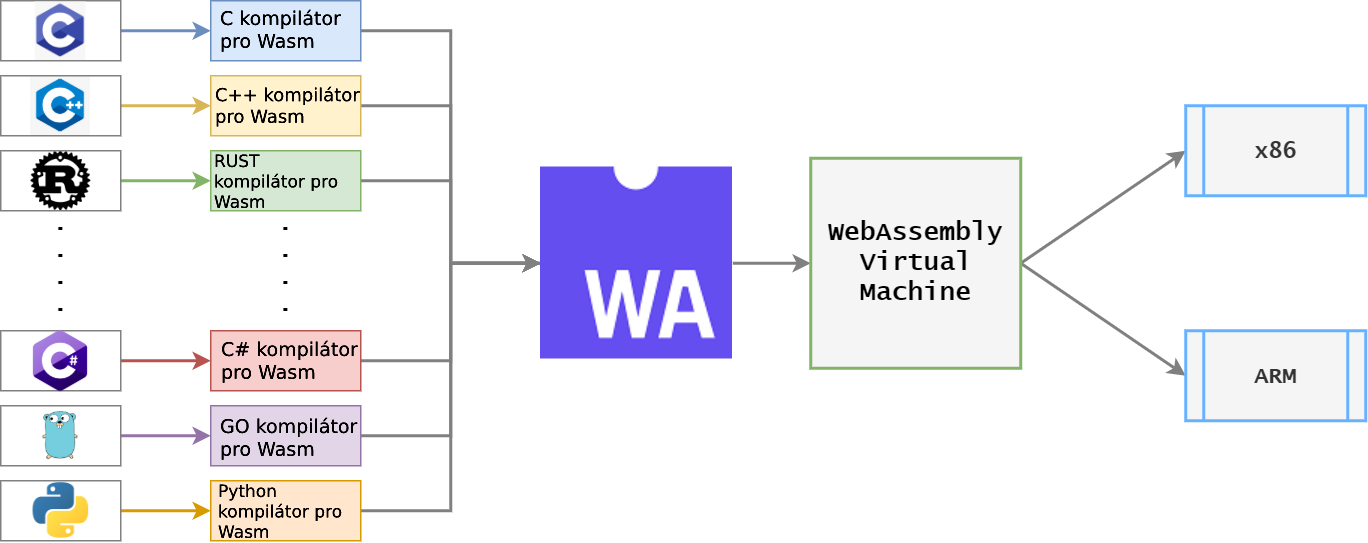
\includegraphics[scale=0.3]{obrazky-figures/PouziteTechnologie/wasm.jpg}
            \caption{Vztah programovacích jazyků k WebAssembly\footnotemark.}
            \label{fig:my_label}
        \end{figure}
        \footnotetext{Vztah programovacích jazyků k WebAssembly --- zdroj viz \url{https://arghya.xyz/images/posts/webassembly/WebAssembly_compile.png} [6. května 2023]}
        
    \subsection{Blazor}
    Blazor je webový framework od společnosti Microsoft pro vytváření interaktivních aplikací. Pomocí Blazor frameworku lze vytvářet Blazor WebAssembly aplikace, což jsou aplikace, jedoucí na straně klienta a Blazor Server aplikace, které jedou na straně serveru, v obou případech se jedná o Blazor framework a mění se pouze, kde je aplikace hostována. Aplikace vytvořené pomocí tohoto frameworku jsou založené na komponentách, kdy každá komponenta je definována jako třída jazyka C\#. Komponenta je prvek uživatelského rozhraní. Pod tím si lze představit stránku, dialogové okno, formulář atd. Blazor komponenty se vytváří pomocí Razor syntaxe, která umožňuje vývojářům kombinovat značkovací jazyk HTML společně s programovacím jazykem C\#~\cite{MicrosoftBlazor}. Tyto komponenty se ukládají s příponou \textit{.razor} jejichž výchozím jazykem je HTML a pomocí znaku "@" se lze přepnout do jazyka C\#.
    
    \subsubsection*{Blazor WebAssembly}
    Blazor WebAssembly je SPA framework pro tvorbu interaktivních aplikací na straně klienta pomocí jazyka C\#. Dle Microsoft dokumentace Blazor WebAssembly aplikace funguje následovně. 
    \begin{itemize}
        \item C\# kód a \textit{.razor} soubory jsou zkompilovány
        \item Zkompilované soubory společně s \textit{.NET} runtime\footnote{Virtuální stroj, který spouští zkompilovaný C\# kód. Obsahuje JIT kompilátor, který zkompiluje zkompilovaný C\# kód (\textit{.ddl} nebo \textit{.exe} soubory) do nativního kódu, který je následně spuštěn počítačem.} jsou staženy do prohlížeče
        \item Blazor WebAssembly v prohlížeči spustí \textit{.NET} runtime jenž spustí aplikaci v javascriptem vytvořeném sandbox\footnote{Vymezené prostředí ve kterém mohou programy jet aniž by měli dopad na vnější systém. Sandbox prostředí se využívá zejména k zajištění bezpečnosti. V prohlížeči se toto prostředí využívá aby se například útočník nedostal k heslům uloženým v prohlížeči, historii prohlížení, cookie souborům atd.} prostředí. Aplikace využívá Javascriptovou interoperabilitu k manipulování s DOM a voláním aplikačního rozhraní prohlížeče.

    \end{itemize}
    
        \begin{figure}[H]
            \centering
            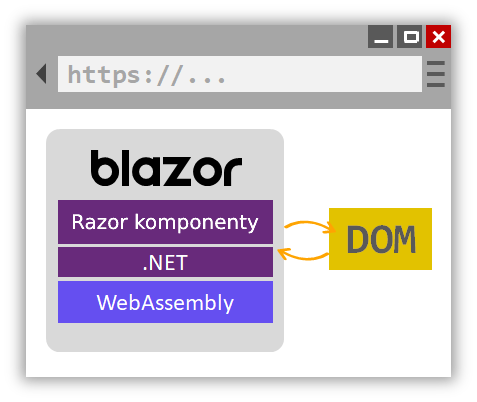
\includegraphics[scale=0.3]{obrazky-figures/PouziteTechnologie/BlazorWasm.png}
            \caption{Grafické znázornění Blazor WebAssembly a DOM\footnotemark.}
            \label{fig:my_label}
        \end{figure}
        \footnotetext{Grafické znázornění Blazor WebAssembly a DOM --- zdroj viz \url{https://learn.microsoft.com/cs-cz/aspnet/core/blazor/?view=aspnetcore-7.0} [6. května 2023]}

    \subsubsection*{Blazor Server}
    Na rozdíl od WebAssembly běžící na straně klienta, Blazor Server je aplikace, běžící na straně serveru a uživatelské prostředí se mění pomocí SignalR spojení~\cite{MicrosoftBlazor} ze serveru. SignalR je open-source knihovna, která slouží primárně k real-time webovým aplikacím. Mezi takové aplikace patří aplikace, které vyžadují frekventované aktualizace ze serveru, konkrétním příkladem jsou hry, mapy, aplikace vyžadující notifikace (sociální, chatovací, emailové, …) a další~\cite{MicrosoftSignalR}. \textit{.NET} runtime se neposílá ze serveru do prohlížeče jako u Blazor WebAssembly, nýbrž zůstává na serveru, kde připraví uživatelské prostředí ve formě HTML na základě uživatelských interakcí, které klient posílá na server a poté pošle zpět klientovi HTML soubor.
    \begin{figure}[H]
        \centering
        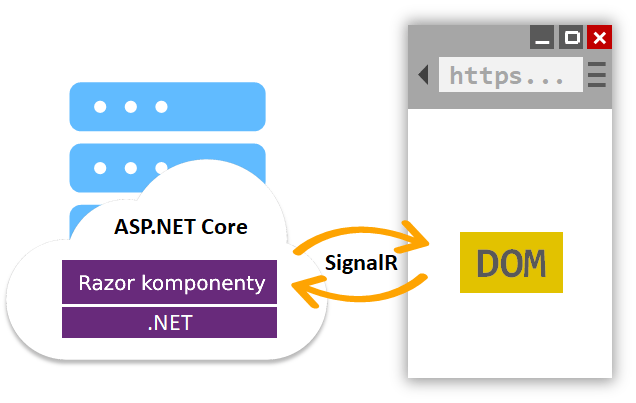
\includegraphics[scale=0.3]{obrazky-figures/PouziteTechnologie/BlazorServer.png}
        \caption{Grafické znázornění Blazor Server a DOM\footnotemark.}
        \label{fig:my_label}
    \end{figure}
    \footnotetext{Grafické znázornění Blazor Server a DOM --- zdroj viz \url{https://learn.microsoft.com/cs-cz/aspnet/core/blazor/?view=aspnetcore-7.0} [6. května 2023]}
    
    \subsection{Použité knihovny}
    \label{sec:UsedLibraries}
    Vývoj aplikací se díky rostoucí poptávce po uživatelské přívětivosti, funkcionalitě a responzivitě stává stále náročnější. Abych dosáhl těmto požadavkům, rozhodl jsem se využít již zmíněné knihovny, které usnadňují vývoj aplikací čímž šetří čas a prostředky vývojářů. Knihovny, které jsem se rozhodl použít jsem zvolil k usnadnění práce s grafickou stránkou aplikace, čímž jsem získal časový prostor, který jsem mohl věnovat funkcionalitě klientské části. Aplikace je postavena na knihovně MudBlazor\footnote{https://mudblazor.com/} a k zobrazení složitějších grafů jsem použil knihovnu ApexCharts\footnote{https://github.com/apexcharts/Blazor-ApexCharts}.
    
    \subsubsection*{MudBlazor}
    MudBlazor je knihovna již připravených \gls{UI} komponent, pro Blazor. Komponentou může být myšleno tlačítko, modální okno, formulář, text, tabulka, atd. Každá komponenta má aplikační rozhraní, kterým lze komponentu jednoduše modifikovat a dosáhnout tak grafických či funkcionálních požadavků. S použitím MudBlazor knihovny lze vytvořit webovou aplikaci, která může být snadno použitelná a responzivní, aniž by vývojář psal veškerý HTML a CSS kód, čímž se stává mocným nástrojem při vývoji. Tato knihovna má open-source licenci a kdokoliv tedy může přispívat při vývoji.
    
    \subsubsection*{ApexCharts}
    ApexCharts je open-source javascriptová knihovna pod licencí MIT, avšak lze ji použít i v Blazoru. V tomto případě se knihovna integruje do aplikace prostřednictvím interop funkcionality. Jinými slovy by se dalo říci, že kód napsaný v Blazoru zavolá javascriptový kód, který se následně spustí v prohlížeči. 
    
    Tato knihovna slouží k zobrazení dat v podobě grafů. Data lze vizualizovat pomocí čárových, sloupcových, plošných, koláčových, kuličkových, svíčkových a mnoho dalších grafů. Dále také poskytuje v těchto grafech určitou funkcionalitu jakou je například zvětšování, zmenšování, pohyb v grafu či stažení grafu v podobě obrázku ve formátu například \textit{.png}. Tyto grafy v podobě komponent mají jednoduché rozhraní, kterým lze upravovat použité barvy či pozadí a dosáhnou tak například lepší čitelnosti nebo aplikace se změnou barevného motivu.

    \subsubsection*{Bogus}
    Bogus je open-source knihovna, která slouží ke generování realistických falešných dat v \textit{.NET} a tedy jazyky C\#, F\# a VB.NET. Knihovna je vysoce konfigurovatelná a lze ji tak použít pro různé specifické užití. Poskytuje snadno použitelné aplikační rozhraní pro generování falešných dat z různých oblastí. Celý seznam dat, které lze pomocí této knihovny vygenerovat je na v souboru Readme.md na githubu\footnote{https://github.com/bchavez/Bogus}, zde uvedu pár dat, která lze s pomocí této knihovny snadno vygenerovat:
    \begin{itemize}
        \item Adresa --- město, ulice, stát, směrovací číslo, číslo domu, zeměpisnou šířku a délku, …
        \item Internet --- emailová adresa, username, \gls{IP} adresa, číslo portu, url adresa, heslo, …
        \item Lidé --- Jméno, příjmení, název práce, popis práce, typ práce, …
        \item Systém --- název souboru, typ souboru, cesta k souboru, verze, Apple Push Token, …
    \end{itemize}
        
\section{Návrh definice aplikačního rozhraní}
    Pro zajištění bezproblémové komunikace mezi serverem a klientem bylo nutné vytvořit aplikační rozhraní a přesné definice objektů pro datový přenos, které jsou použity k přesunu informací ze serveru na klienta a k jednoduché manipulaci s daty při následné vizualizaci. Jelikož cílem této práce je pouze data vizualizovat a nikoliv modifikovat, přidávat či mazat, tak jediné dotazy, které server zpracovává jsou dotazy typu GET. 
    
    Objekty pro datový přenos jsou navrženy pro přesun dat ze serveru na klienta s ohledem na co největší efektivitu a jednoduchost zpracování na straně klienta. Při návrhu objektů pro datový přenos jsem se inspiroval u již existujících nástrojů, u kterých jsem analyzoval jaká data a v jaké podobě se zobrazují na konkrétních pohledech. Po následné konzultaci s vedoucím práce jsem došel k finální struktuře aplikačního rozhraní a vytvořeným návrhem objektům pro datový přenos, jejichž tvorbu popisuji v následujících subsekcích.

    \subsection{Struktura aplikačního rozhraní}
        Nástroj Xplico umožňuje uživateli vytvářet případy obsahující zachycenou komunikaci. Tímto jsem se inspiroval a rozhodl se vytvořit stejnou funkcionalitu taktéž. Vytvoření případů umožní uživatelům snadněji a efektivněji analyzovat zachycenou komunikaci v rámci jednoho vyšetřovacího případu. Pro dosažení maximální efektivity při přenosu dat mezi serverem a klientem bylo nutné pečlivě navrhnout aplikační rozhraní. Základní strukturu aplikačního rozhraní vizualizuje obrázek~\ref{fig:APICaseDesign}, který popisuje základní navržení aplikačního rozhraní, nikoliv konkrétní koncové body. Koncových bodů je v rámci aplikačního rozhraní více (např. kvůli filtrování dat).
        
        Případ slouží ke sdružení veškerých zachycených spolu souvisejících dat. To může být zejména vhodné pokud má vyšetřovatel v rámci jednoho vyšetřujícího případu více zachycených komunikací, které chce analyzovat zároveň. Koncový bod "Obsah" poskytuje informace o případu (datum první a poslední zachycené komunikace, počet zachycených komunikací, atd.). Zachycení reprezentuje konkrétní zachycenou komunikaci a informace o ní. Zobrazenou komunikaci v rámci celého případu jsem se rozhodl zobrazovat dle vrstev referenčního modelu ISO/OSI, konkrétně na vrstvách L3, L4 a L7 a také dle aplikačních protokolů \gls{HTTP}, \gls{DNS}, \gls{SMTP} a \gls{POP}. Zachycenou komunikaci nad protokolem \gls{HTTP} jsem dále rozdělit na \gls{HTTP} odpovědi a \gls{HTTP} dotazy a komunikaci nad protokolem \gls{SMTP} a \gls{POP} na komunikaci ze serveru a od klienta.
        
        \begin{figure}[H]
            \centering
            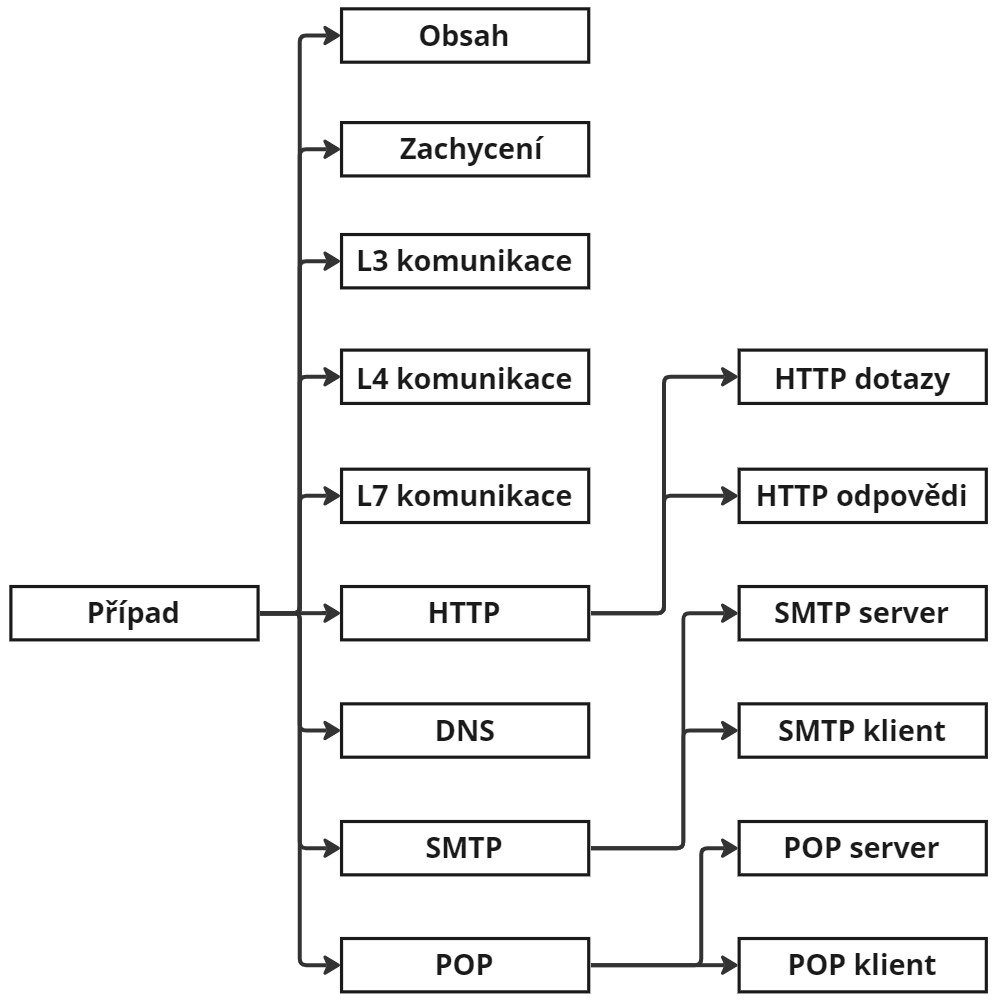
\includegraphics[scale=0.3]{obrazky-figures/Implementace/NavrhAPI/APIStructure.jpg}
            \caption{Navržená základní struktura aplikačního rozhraní.}
            \label{fig:APICaseDesign}
        \end{figure}

    \subsection{Objekty pro datový přenos}
        V této subsekci popíšu jak jsem modely vytvářel. Pro zobrazování kolekcí zpráv stejného typu (např. kolekce všech případů) jsem vytvořil \textit{"List"} model, který obsahuje pouze některé informace o konkrétní zprávě. Tento přístup jsem zvolil, abych uživateli vytvořil možnost se postupně zanořovat v aplikaci a zobrazovala se mu pouze ta data, o která má zájem. Zároveň tak šetřím data, která je nutná přeposlat ze serveru na klienta a datový přenos je tak rychlejší.
        
        K lepšímu \gls{UX} jsem se rozhodl implementovat stránkování při zobrazovaní kolekce vizualizovaných dat. Stránkování dat umožňuje uživateli rychlý a efektivní přístup k velkým kolekcím dat. Z tohoto důvodu jsem potřeboval uchovávat informaci, na které stránce se uživatel nachází a také kolik dat se má na stránce zobrazit, jelikož to je jedna z možností, které si může uživatel určit. To jsem vyřešil vytvořením objektů pro datový přenos se suffixem \textit{"PageQueryResultDTO"}, který slouží jako obálka obsahující tyto informace o stránkování a kolekci všech zpráv stejného typu.

        K zobrazení jedné konkrétní zprávy jsem vytvořil \textit{"Detail"} model, jenž obsahuje všechna dostupná data o zprávě. Tento model už se ze serveru na klienta odesílá samostatně a tedy nedochází ke zbytečnému zahlcení sítě, které by vznikalo pokud bych některá přijatá data ze serveru nezobrazoval. Tyto modely jsem použil například při zobrazení zpráv na vrstvě L3, L4 a L7.
        
\section{Návrh uživatelského prostředí}
Po navržení aplikačního rozhraní, jsem byl schopen přejít na návrh samotného uživatelského prostředí a vizualizovat jednotlivé stránky aplikace, celkový vzhled a jak bude možné aplikaci ovládat. Nejprve jsem vytvořil jednoduché drátové modely, které mi sloužili k rozvržení aplikace tak aby byla pro uživatele srozumitelná, jednoduše použitelná a nápomocná při čtení zobrazených dat. Po vytvoření těchto drátových modelů jsem vytvořil grafický návrh, který už reprezentoval vzhled výsledné aplikace.

Návrh drátových a grafických modelů před samotným vývojem je velice běžné jelikož šetří čas a zdroje potřebné k vývoji aplikace. Vytvoření těchto modelů není tak časově náročné jako samotný vývoj. Lze tak rychle vizualizovat vzhled a použitelnost výsledného celku a zjistit tak případné nedostatky či chyby. Modely je možné následně předělat či upravit tak, aby vyhovovaly veškerým požadavkům a aplikace byla pro koncového uživatele jednoduše ovladatelná a uživatelsky přívětivá.

    \subsection{Drátové modely}
    Jedná se o velice jednoduchý model, který by měl být tvořen pouze pomocí čar a textu. Účelem je rychle vizualizovat rozložení prvků aplikace, které pak slouží grafikům při návrhu grafických UI modelů, programátorům při vytváření znovupoužitelných komponent pro zjednodušení vývoje aplikace, atd. Při tvorbě těchto modelů často vznikají nové nápady na vylepšení aplikace. Tyto modely mohou být také součástí smlouvy, aby se zabránilo případným neshodám při dodání aplikace zákazníkovi.
    
    Pro tvorbu drátových modelů jsem použil nástroj Miro. Vytvořil jsem si šablony webového prohlížeče a poté pomocí elektronické tužky jsem do těchto šablon kreslil. Drátové modely jsem navrhoval na základě již vytvořeného aplikačního rozhraní a zároveň jsem se inspiroval jinými nástroji (Xplico, NetworkMiner, …). Chtěl jsem vytvořit nástroj, který bude zobrazovat data ze zachycené komunikace a zároveň uživateli poskytne možnost agregace vybraných dat a poskytne uživateli agregované hodnoty ze všech právě zobrazených dat na stránce v podobě grafů. 

    Abych ušetřil čas při vytváření drátových modelů, rozhodl jsem se je vytvořit genericky. Namísto vytváření drátového modelu pro každou stránku jsem vytvořil generickou verzi pro stránku zobrazující konkrétní zprávu, kolekci všech zpráv a další informace o zobrazené kolekci (grafy, agregovaná data a podezřelá slova v obsahu zprávy).


    Na obrázku~\ref{fig:wireframeListPage} je konečná verze drátového modelu pro zobrazení kolekce zpráv. Obsahuje tabulku, v níž budou data zobrazena společně s možností vyhledávání. Pod tabulkou se nachází otevíratelné panely, obsahující dodatečnou funkcionalitu a informace nad kolekcí.
    \begin{figure}[H]
        \centering
        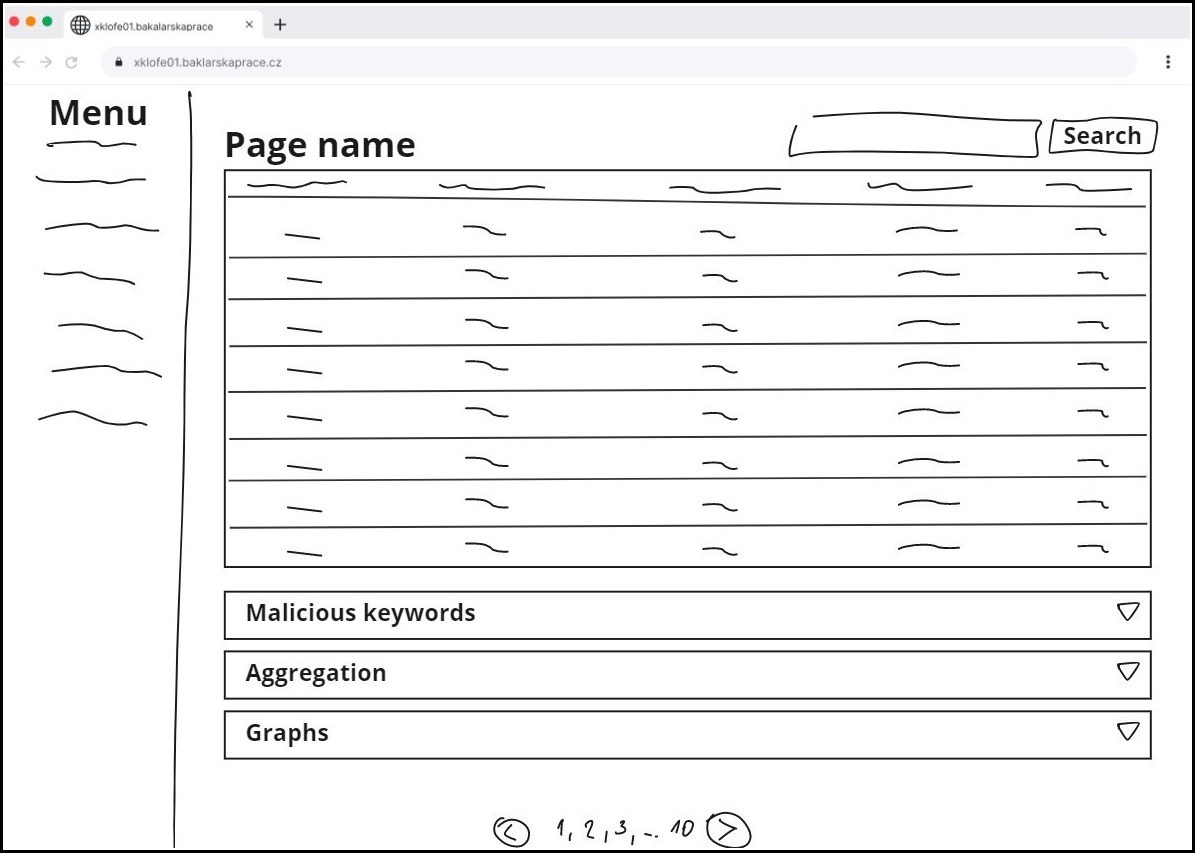
\includegraphics[scale=0.25]{obrazky-figures/NavrhUXUI/ListPage.jpg}
        \caption{Drátový model vizualizující rozložení stránky zobrazující kolekci zachycených zpráv, včetně možnosti agregace dat, vyhledávání a stránkování.}
        \label{fig:wireframeListPage}
    \end{figure}

    Otevřené panely lze vidět na obrázku~\ref{fig:wireframeListPagePanels}. V panelu s názvem \textit{"Malicious keywords"} se nachází seznam zpráv, které ve svém obsahu mají podezřelá slova. Tato funkcionalita může vyšetřovali nejen ušetřit čas při prohledávání zpráv, ale zejména ho upozorní na existenci zprávy s podezřelým obsahem.

    Další panel jenž nese nadpis \textit{"Aggregation"} slouží k agregaci dat podle odesílatele. Při zadání jména do pole pro vkládání textu se agregují informace o daném uživateli z kolekce právě zobrazených zpráv. Takovými informacemi jsou například celkový počet zpráv, které uživatel napsal, odeslané přílohy, adresáti atd. Poslední panel s nadpisem \textit{"Graphs"} obsahuje grafy vytvořené nad právě zobrazenou kolekcí.

        Poslední drátový model~\ref{fig:wireframeDetailPage}, který zde zmíním je model pro zobrazení konkrétní zprávy. Na úvod stránky jsem vložil základní informace o zprávě a poté jsem jednotlivé části rozdělil a vložil do otevíracích panelů. Takto se uživatel může jednoduše zanořit a nezobrazují se mu informace, které nechce vidět. Konkrétním příkladem je například obsah emailové zprávy, který může být značně rozsáhlý a zabírat tak poměrně velkou část celé stránky.
        
    \begin{figure}[H]
        \centering
        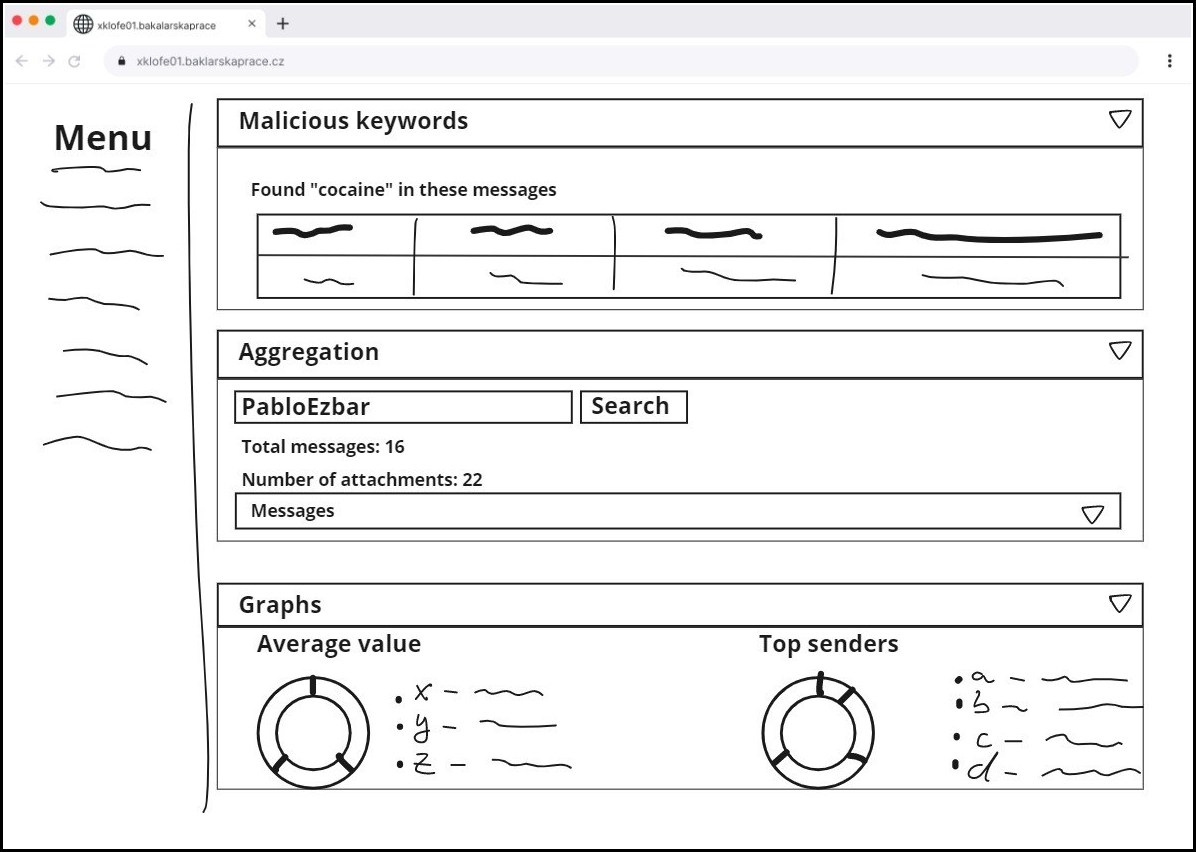
\includegraphics[scale=0.3]{obrazky-figures/NavrhUXUI/ListPageDetail.jpg}
        \caption{Drátový model reprezentující rozložení stránky zobrazující kolekci zachycených zpráv s otevřenými záložkami k zobrazení grafů, agregaci dat konkrétního uživatele a zpráv obsahujících podezřelé slova.}
        \label{fig:wireframeListPagePanels}
    \end{figure}


    
    \begin{figure}[H]
        \centering
        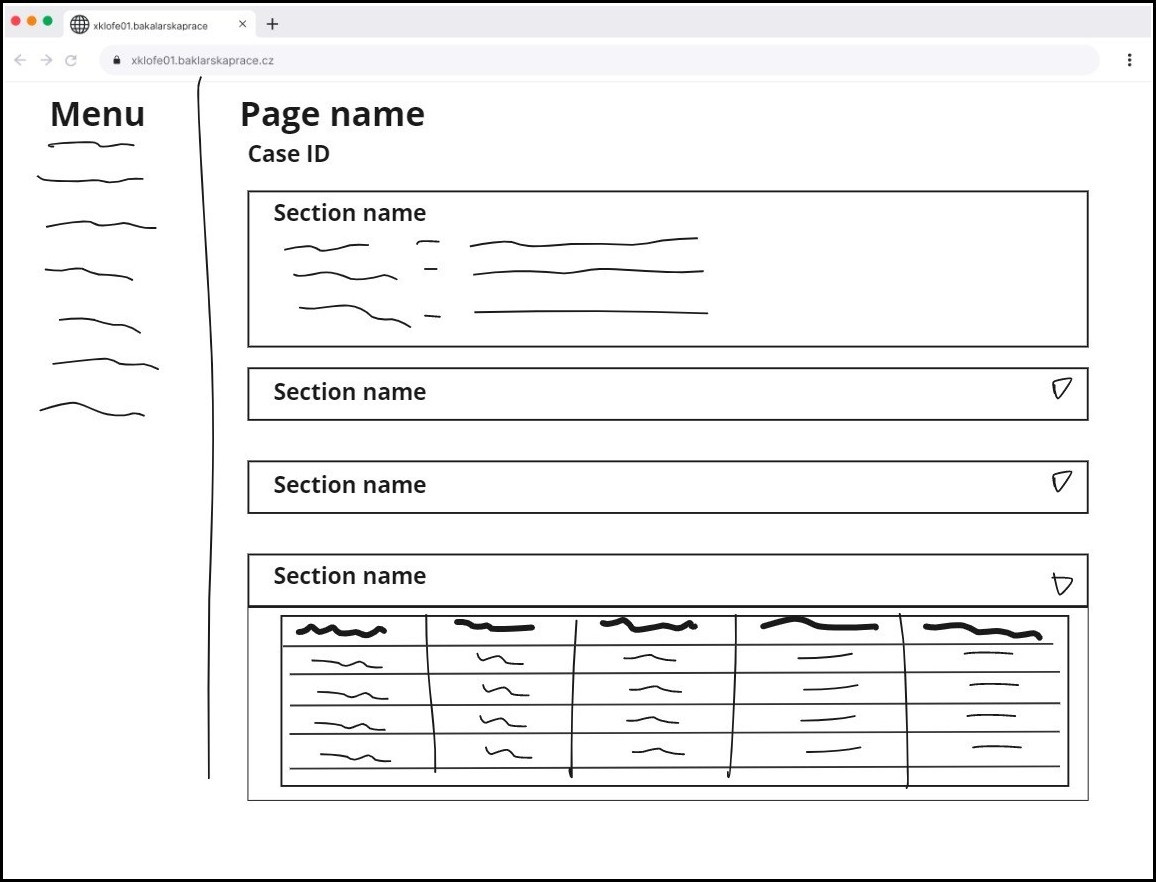
\includegraphics[scale=0.3]{obrazky-figures/NavrhUXUI/DetailPage.jpg}
        \caption{Drátový model reprezentující rozložení stránky zobrazující detailní informace konkrétní zprávy v otevíratelných panelech.}
        \label{fig:wireframeDetailPage}
    \end{figure}
    
    \subsection{Grafický návrh}
    Poté, co jsem vytvořil drátové modely, jsem si vytvořil grafické modely jednotlivých stránek pomocí nástroje Figma\footnote{Figma je vektorový grafický editor zaměřující se na \gls{UX} a \gls{UI}}. Stáhl jsem si předlohu prohlížeče a začal tvořit pro každou stránku samostatný model, který reprezentoval konečný vzhled stránky. 

    K urychlení práce jsem si vytvářel komponenty, ze kterých jsem tvořil instance a ty vkládal do jednotlivých stránek. To vytvořilo časovou úsporu, jelikož kdykoliv jsem potřeboval některou z komponent změnit, stačilo změnit pouze rodičovskou neboli referenční a všechny její instance se automaticky změnily taktéž. Podle těchto modelů jsem následně programoval aplikaci. Přestože jsem však vytvářel modely tak aby vizualizovali výslednou podobu aplikace, při její implementaci jsem se občas od modelů odchýlil, důvodem bylo zjednodušení implementace.
    
    Na obrázku~\ref{fig:SmtpClientDetail} můžete vidět \gls{UI} model, podle kterého jsem vytvářel stránku pro zobrazení detailních informací o zachycené komunikace elektronické pošty nad protokolem \gls{SMTP}. Informace jsou členěny do sekcí z důvodu lepší orientace uživatele na stránce - obálka ("\textit{Envelope}"), zpráva (\textit{"Email"}) a přílohy (\textit{"Attachments"}). Obrázek~\ref{fig:L7ListUIModel} vizualizuje návrh stránky pro zobrazení kolekce zachycených zpráv na vrstvě L7. Na místo konkrétních hodnot jsem při vytváření těchto modelů použil pouze popis reprezentující datový typ hodnoty, která bude na daném místě.

    \begin{figure}[H]
        \centering
        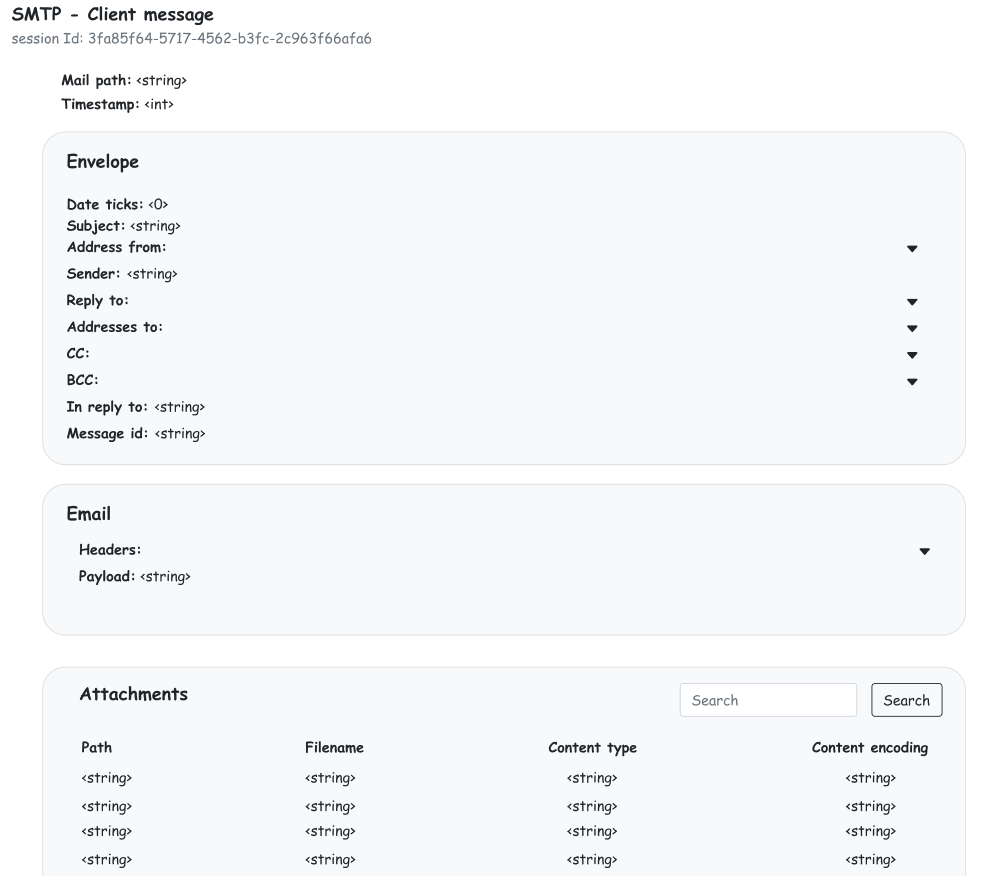
\includegraphics[scale=0.5]{obrazky-figures/NavrhUXUI/UIModels/SmtpClientDetail.png}
        \caption{\gls{UI} Model zobrazující stránku s detailními informacemi o zachycené elektronické zprávy nad protokolem \gls{SMTP}.}
        \label{fig:SmtpClientDetail}
    \end{figure}

    \begin{figure}[H]
        \centering
        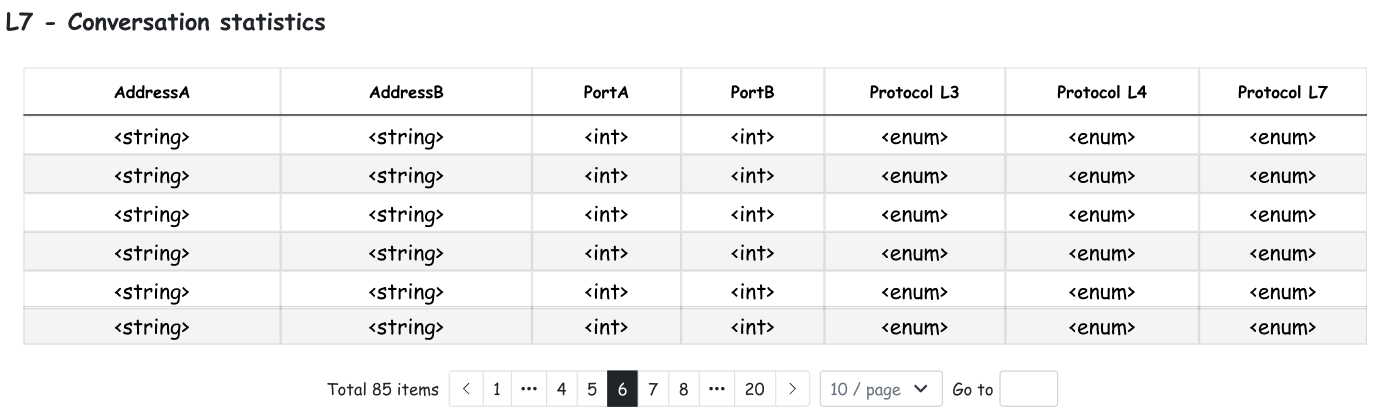
\includegraphics[scale=0.45]{obrazky-figures/NavrhUXUI/UIModels/L7List.png}
        \caption{\gls{UI} Model zobrazující stránku s kolekcí zachycené komunikace na vrstvě L7.}
        \label{fig:L7ListUIModel}
    \end{figure}



\section{Tvorba webové aplikace}
    Následující část popisuje samotnou implementaci, jejichž úspěšný výsledek závisí na předešlé práci a to zejména na nastudované teorii, drátových a grafických modelech ale také na praktických zkušenostech nabitých v dosavadním studiu. 
    
    Implementaci jsem rozdělil do 3 částí. Sdílená část, která slouží k uchování modelů, které jsou společné jak pro serverovou, tak pro klientskou část. Serverová část, byla vytvořena k otestování komunikace s klientskou částí a zároveň jako zdroj dat. Jelikož se tato práce zabývá vizualizací dat a tedy klientské části, vytvořil jsem serverou část pouze tak, aby odpovídala na dotazy a nedbal jsem zvýšené pozornosti na její rozšiřitelnost v budoucnu. Poslední částí je klientská část. Tato část už se zabývá samotnou vizualizací dat. Bylo zapotřebí vytvořit jednotlivé stránky a znovupoužitelné komponenty, abych zbytečně nekopíroval stejný kód. Při vytváření komponent a stránek jsem použil knihovny, abych ušetřil čas psaním HTML a CSS kódu a mohl se věnovat funkcionalitě a zlepšení \gls{UX} aplikace. Použité knihovny jsou detailně popsané v předešlé sekci~\ref{sec:UsedLibraries}.

    \begin{figure}[H]
        \centering
        
\includegraphics[scale=0.12]{obrazky-figures/Implementace/AppStructure.jpg}
        \caption{Vizualizace struktury projektu, šipky ukazují závislost.}
        \label{fig:my_label}
    \end{figure}


    
    \subsection{Serverová část}
        Serverová část byla vytvořena pouze k otestování správné funkčnosti komunikace v klientské části. Jelikož serverová část není hlavním tématem této práce, nebyl z tohoto důvodu kladen důraz na případnou rozšiřitelnost v budoucnu. Napsaný kód tedy nemusí splňovat některá doporučení při psaní čistého kódu. 

        Serverovou část jsem vygeneroval z již vytvořeného návrhu aplikačního rozhraní pomocí nástroje Swagger. Tento nástroj vygeneruje jednoduchou kostru skládající se z kontrolerů zastávající komunikaci se serverem a objekty pro datový přenos. Vygenerovaný kód vyžaduje úpravy ke správné funkčnosti serveru, avšak dříve než jsem začal upravovat tento vygenerovaný kód jsem začal vytvářet testovací data jejichž tvorba je popsána níže v této subsekci.
                
        Vygenerované kontrolery obsahují funkce, které nevrací žádná data. Z tohoto důvodu bylo nutné vygenerovaný kód upravit tak, aby jednotlivé funkce vracely patřičná data. Dalším krokem byla úprava objektů pro datový přenos. Jelikož jsou modely použity i v rámci klientské části, rozhodl jsem se je vyjmout z vygenerovaného projektu a vytvořit pro ně nový projekt, na který jsem poté vytvořil závislost jak ze serverové, tak z klientské části.

        \subsubsection*{Testovací data}
            Pro každý typ komunikace (\gls{POP} server, \gls{POP} client, \gls{HTTP} Response, atd.) jsem vytvořil samostatnou statickou třídu, ve které jsem vytvořil kolekci v podobě seznamu neboli listu. V této kolekci jsem následně uchovával jak ručně vytvořená, tak i vygenerovaná data. Některá data jsem vytvořil ručně, abych mohl replikovat testovací příklad použitý k vytvoření případů užití ke zmapování a prozkoumání konkurenčních nástrojů (Xplico, NetworkMiner). V tomto případě jsem si stáhl \textit{.pcap} soubor testovacího případu (více v sekci~\ref{sec:XplicoNetworkMiner}), který jsem si otevřel v nástroji Wireshark a ručně vytvářel jednotlivé objekty pro datový přenos z vyčtených dat. 
            
            Poté, co jsem měl vytvořená potřebná data k replikaci testovacího příkladu, jsem použil knihovnu Bogus. Pomocí této knihovny jsem rychle vytvořil více než 1000 falešných dat, která slouží k zaplnění aplikace daty a otestování implementované funkcionality aplikace jako je například filtrování, agregace dat, zobrazení grafů atd.
            
            Generování falešných dat (viz výpis~\ref{lst:fakerGenerating}) s nástrojem Bogus probíhá tak, že pro každou třídní proměnnou se nastaví kolekce ze které se pro tuto proměnnou bude náhodně vybírat hodnota. Nástroj Bogus má rozsáhlý výběr dat, která lze použít avšak v mém případě bylo k otestování aplikace nutné aby se některá data opakovala (IP adresy, emailové adresy, ID relací, atd.). Z tohoto důvodu jsem vytvořil jednu statickou třídu, jejichž účelem je uchování mnou vytvořených kolekcí dat (IP adres, emailových adres, ID relací, atd.), které jsem využíval při tvorbě všech generovaných falešných dat pro jednotlivé objekty pro datový přenos.


\begin{lstlisting}[numbers=left, firstnumber=1, caption={Ukázka tvorby falešných dat pro objekt sloužící k datovému přenosu „PopServerMessageDTO“ pomocí nástroje Bogus.}, label={lst:fakerGenerating}]
var PopServerMessage = new Faker<PopServerMessageDTO>()
  .RuleFor(o => o.SessionId, f => f.PickRandom(SharedDTOsSeeds.GuidArray))
  .RuleFor(o => o.Reply, f => f.Random.Enum<PopServerMessageDTO.ReplyEnum>())
  .RuleFor(o => o.Description, f => f.Commerce.ProductDescription())
  .RuleFor(o => o.Payload, f => f.Lorem.Paragraphs(randomNum.Next(1, 5)))
  .RuleFor(o => o.Envelope, f => SharedDTOsSeeds.EmailEnvelopeFaker.Generate(1)[0])
  .RuleFor(o => o.Email, f => SharedDTOsSeeds.EmailMessageFaker.Generate(1)[0])
  .RuleFor(o => o.MailPath, f => f.PickRandom(SharedDTOsSeeds.EmailPath))
  .RuleFor(o => o.Timestamp, f => (int)DateTime.UtcNow
    .Subtract(f.Date.Between(new DateTime(1990, 1, 1), new DateTime(2022, 1, 1)))
    .TotalSeconds)
  .RuleFor(o => o.Attachments, f => SharedDTOsSeeds.EmailAttachmentFaker.Generate(randomNum.Next(0, 15)));

PopServerMessageListSeed.Items = PopServerMessage.Generate(NumberOfPopClientMessages);
\end{lstlisting} 

    \subsection{Klientská část}
      Vytvoření vizualizační aplikace, která umožní uživatelům snadno a rychle pracovat s daty je hlavním tématem této práce a při vývoji jsem kladl důraz na čitelnost a udržitelnost kódu, abych zajistil snadnou rozšiřitelnost aplikace v budoucnu. Pro dosažení tohoto cíle jsem vytvořil dva projekty: klientskou Blazor aplikaci a komunikační knihovnu. V komunikační knihovně je obsažena veškerá komunikační logika mezi aplikačním rozhraním na serveru a Blazor aplikací, zatímco klientská aplikace, se kterou interaguje uživatel se zaměřuje pouze na vizualizaci dat.

      Oddělením komunikační logiky od klientské aplikace jsem zajistil, že každý projekt má pouze jednu odpovědnost a tedy jeden důvod k existenci. Klientská aplikace tak obsahuje pouze kód související s vizualizací dat a uživatelským rozhraním. Kromě výhod jako znovupoužitelnost, testovatelnost a udržitelnost, tento přístup také zajišťuje snadnější údržbu a modulárnost kódu, což v budoucnu umožní jednodušší rozšíření aplikace.

    \subsubsection*{Komunikační knihovna}
        Komunikační knihovna zajišťuje veškerou komunikaci se serverem a je tedy komunikačním prostředníkem mezi klientskou aplikací a aplikačním rozhraním na serveru. Díky tomu, že veškerá komunikační logika je oddělena do samostatného projektu, lze jednoduše modifikovat a rozšiřovat kód bez zásadních změn na klientskou aplikaci. Komunikační knihovna vytváří abstrakci a chrání klientskou aplikaci před případnými změnami. Při vytváření komunikační knihovny jsem postupoval následovně:

        \begin{itemize}
            \item Vygenerování aplikačního klienta --- aplikačního klienta jsem vygeneroval pomocí nástroje NSwagStudio\footnote{NSwagStudio --- open-source nástroj pro generování aplikačních klientů a serverového kódu na základě REST aplikačního rozhraní využívající Swagger (OpenAPI) specifikaci. Nástroj NSwagStudio má grafické rozhraní a umožňuje tak jednoduchou interakci s uživatelem. NSwagStudio umí generovat kód nejen v jazyce C\# ale i v jazyce typescript.}. Aplikační klient slouží ke komunikaci se serverem skrze jednotlivé koncové body aplikačního rozhraní. Vygenerovaný klient obsahuje funkci pro každý koncový bod a interně provádí serializaci a deserializaci dat. Díky tomu je komunikace se serverem velmi jednoduchá, stačí pouze zavolat patřičnou funkci a ta provede potřebné požadavky na serveru.
            \item Vytvoření fasád --- vytvořením fasád mezi generovaným aplikačním klientem a samostatnou klientskou aplikací jsem mezi nimi zjednodušil komunikaci a skryl složitost aplikačního klienta před klientskou aplikací. Generovaný kód nemusí být lehce čitelný či modifikovatelný a z tohoto důvodu je vhodné vytvořit pomocí fasády rozhraní vyšší úrovně. Dále vytvořením fasád, se vytvořila vrstva abstrakce, která usnadňuje případné změny v budoucnu, které tak nemusí ovlivnit klientskou aplikaci. Pokud by byl aplikační klient nějakým způsobem modifikován či zcela nahrazen, jediným místem v kódu, na které by měla případná změna vliv, by byla právě ona fasáda. Pokud by tedy rozhraní fasády zůstalo po modifikaci stejné, klientská aplikace by nebyla třeba jakkoliv modifikovat.
        \end{itemize}
        
    \subsubsection*{Blazor aplikace}
        Blazor aplikaci jsem vyvíjel pomocí grafických návrhů, které jsem měl již vytvořené. Nicméně přestože jsem strávil poměrně dost času tvorbou těchto návrhů, během vývoje jsem přicházel s nápady jak aplikaci vylepšit. Nyní popíšu jak jsem postupoval při tvorbě stránek a ukážu některé změny oproti grafickému návrhu.

        Prvotním krokem při vytváření klientské aplikace byla instalace knihoven MudBlazor a ApexCharts viz~\ref{sec:pouziteTechnologie}. Instalace těchto knihoven proběhla velice snadno díky řádně zpracované dokumentaci na oficiálních stránkách. Na knihovně MudBlazor je postavena celá aplikace a z toho důvodu byla její instalace nutná hned na začátku. Dále jsem pokračoval vytvářením \gls{UI} jednotlivých stránek a následně jejich funkcionality. Pro funkcionalitu jenž se opakovala na více stránkách a bylo to možné, jsem vytvořil samostatnou komponentu, abych nevytvářel stejný kód na více místech. 
        
        Díky již vytvořeným grafickým modelům a knihovnou s připravenými UI komponentami byla tvorba stránek velice jednoduchá. Nejprve jsem začal se stránkou pro výběr případů. Pokud uživatel nemá vybraný žádný případ, jeho přístup v aplikaci je limitovaný pouze na hlavní stránku a stránku s kolekcí případů. Pokud chce uživatel přejít na stránku, která vyžaduje vybraný případ, je odkázán na stránku s kolekcí případů, na které se objeví informační hláška, která uživatele informuje o problému.

        \paragraph{Stránky obsahující kolekce zachycených zpráv}
        Následně jsem začal vytvářet stránky obsahující kolekce zpráv. Všechny tyto stránky obsahují tabulku, jenž zobrazuje data ze serveru a nějakou formu agregovaných dat, nejčastěji v podobě grafů. V každé tabulce lze filtrovat právě zobrazená data díky jednoduchému rozhraní, které vizualizuje obrázek~\ref{fig:tableFilter}. 

        \begin{figure}[H]
            \centering
            
\includegraphics[scale=0.3]{obrazky-figures/Implementace/Blazor/TableFiltration.png}
            \caption{Rozhraní pro specifikování filtrování nad daty zobrazené v tabulce.}
            \label{fig:tableFilter}
        \end{figure}
        Ve většině tabulek v rámci celé aplikace lze vytvořit libovolný počet filtrů, přičemž si uživatel vybere sloupec nad kterým se bude filtr provádět, hledanou hodnotu a operátor který závisí na datovém typu sloupce (string, int, date, …) a dle datového typu nabídne patřičné operátory. Tuto funkcionalitu vizualizuje obrázek~\ref{fig:tableFilterOperators}, na kterém můžete vidět možnost výběru operátorů dle datového typu hodnoty ve vybraném sloupci. Z obrázku~\ref{fig:tableFilterOperators} lze vidět, že uživatel má rozsáhlé možnosti filtrování dat a tedy zobrazení pro uživatele relevantních dat.
        \begin{figure}[H]
            \centering
            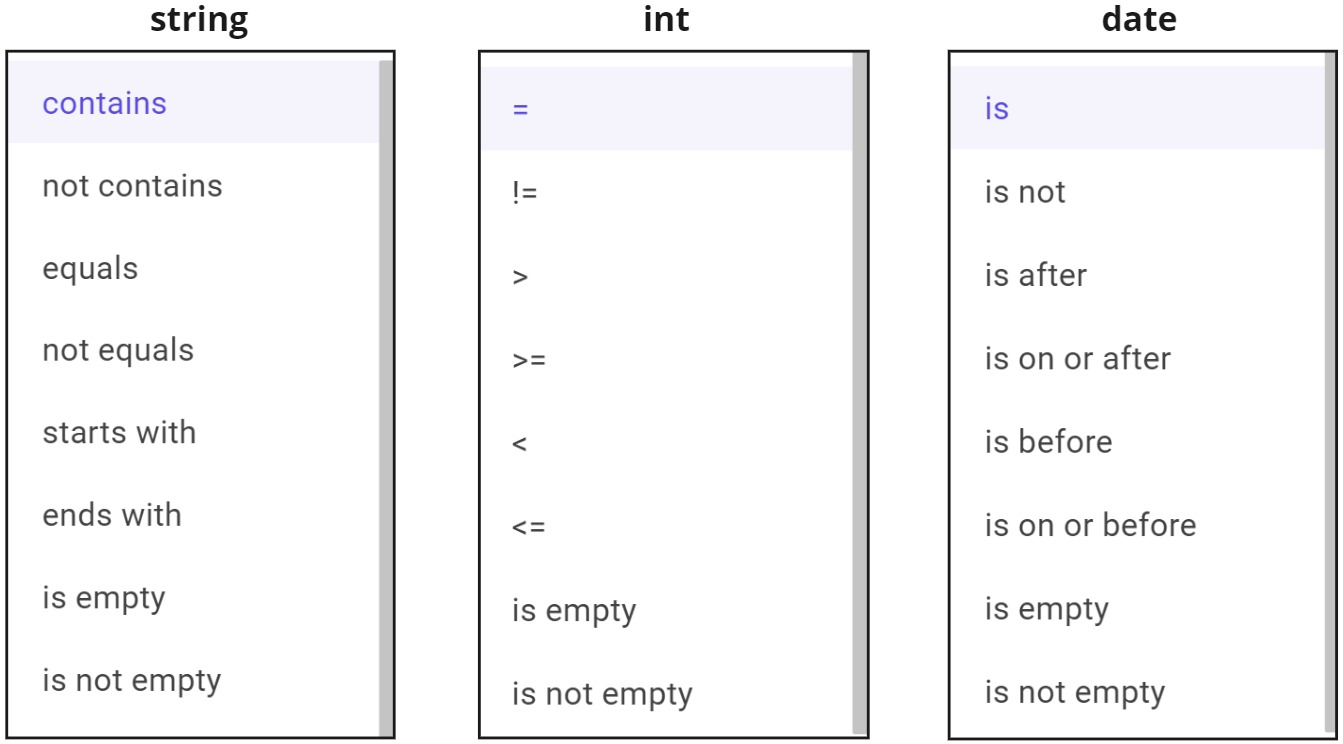
\includegraphics[scale=0.22]{obrazky-figures/Implementace/Blazor/TableFilterOperators.jpg}
            \caption{Kolekce operátoru, při vytváření nového filtru nad tabulkou, ze kterých si uživatel vybere operátor k filtraci dat v tabulce. Dle vybraného sloupce a datového typu hodnot v něm se uživateli zobrazí určitá kolekce operátorů.}
            \label{fig:tableFilterOperators}
        \end{figure}

        Pro každou kolekci jsem vytvořil graf nad daty, jenž jsem považoval za vhodný ke grafickému zobrazení. Nejčastěji se jednalo o maxima, minima, nejčastější hodnoty, zobrazení všech nebo konkrétních zpráv v čase atd. Ukázku zobrazení zpráv v čase můžete vidět na snímku~\ref{fig:tableFilterOperators}. Jedná se o komponentu z knihovny ApexCharts zobrazující zprávy v čase uživatelem vybraných odesílatelů. Graf lze stáhnout v podobě \textit{.svg}, \textit{.png} či \textit{.csv}. Celkově jsem si uvědomoval, že grafické zobrazení dat může být pro uživatele mnohem srozumitelnější a názornější než pouhé zobrazení čísel. Proto jsem se snažil vytvořit grafy, které budou plnit svůj účel a zároveň budou esteticky příjemné a snadno čitelné.

        \begin{figure}[H]
            \centering
            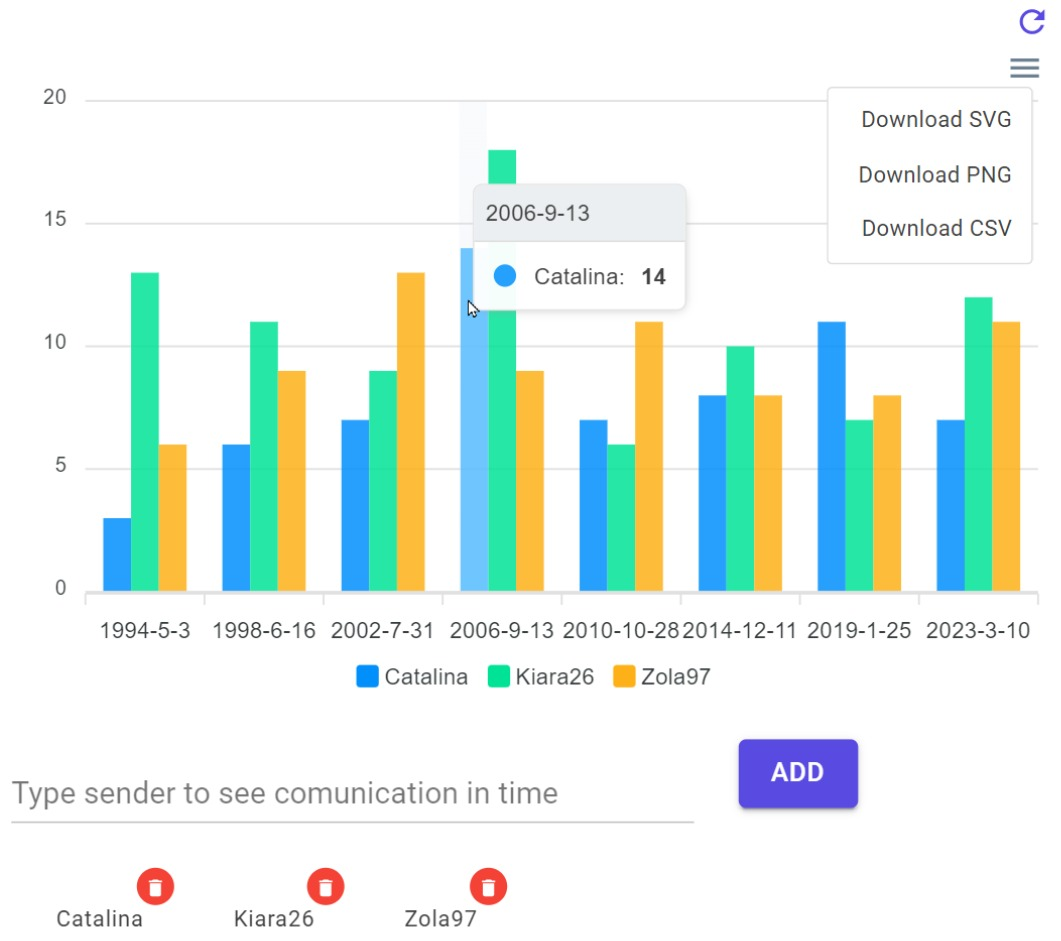
\includegraphics[scale=0.25]{obrazky-figures/Implementace/Blazor/chart.jpg}
            \caption{Graf zobrazující zachycené zprávy v čase, uživatelem vybraných odesílatelů.}
            \label{fig:tableFilterOperators}
        \end{figure}

        Na některých stránkách aplikace umožňuji uživatelům provádět agregaci dat, tedy zobrazit zprávy, které obsahují určitá podezřelá klíčová slova nebo informace o konkrétním odesílateli. Pro tyto účely jsem v aplikaci nastavil výchozí klíčová slova, která jsem považoval za nejvhodnější pro detekci problematických zpráv. Jedná se například o názvy nelegálních drog, zbraní, slova týkající se násilí atd. Pokud některá ze zpráv obsahuje některé ze slov, zobrazí se v nové tabulce. 
        
        Pokud aplikace zachytí zprávu obsahující některé z těchto klíčových slov, zobrazí se uživateli v nové tabulce, aby mohl být upozorněn na potenciálně podezřelou zprávu. Uživatel má také možnost přidávat svá vlastní klíčová slova, která by mohla být pro něj relevantní a odstraňovat jak svá vlastní, tak i výchozí klíčová slova. 
        
        Tato funkce je pro vyšetřovatele velmi užitečná, protože umožňuje rychle identifikovat potenciálně podezřelé zprávy bez nutnosti procházet ručně celým seznamem zachycených zpráv. To může být velmi časově náročné, zejména v případech, kdy je k dispozici velké množství dat. Díky této funkci se tak proces vyšetřování může urychlit a zefektivnit.

        \begin{figure}[H]
            \centering
            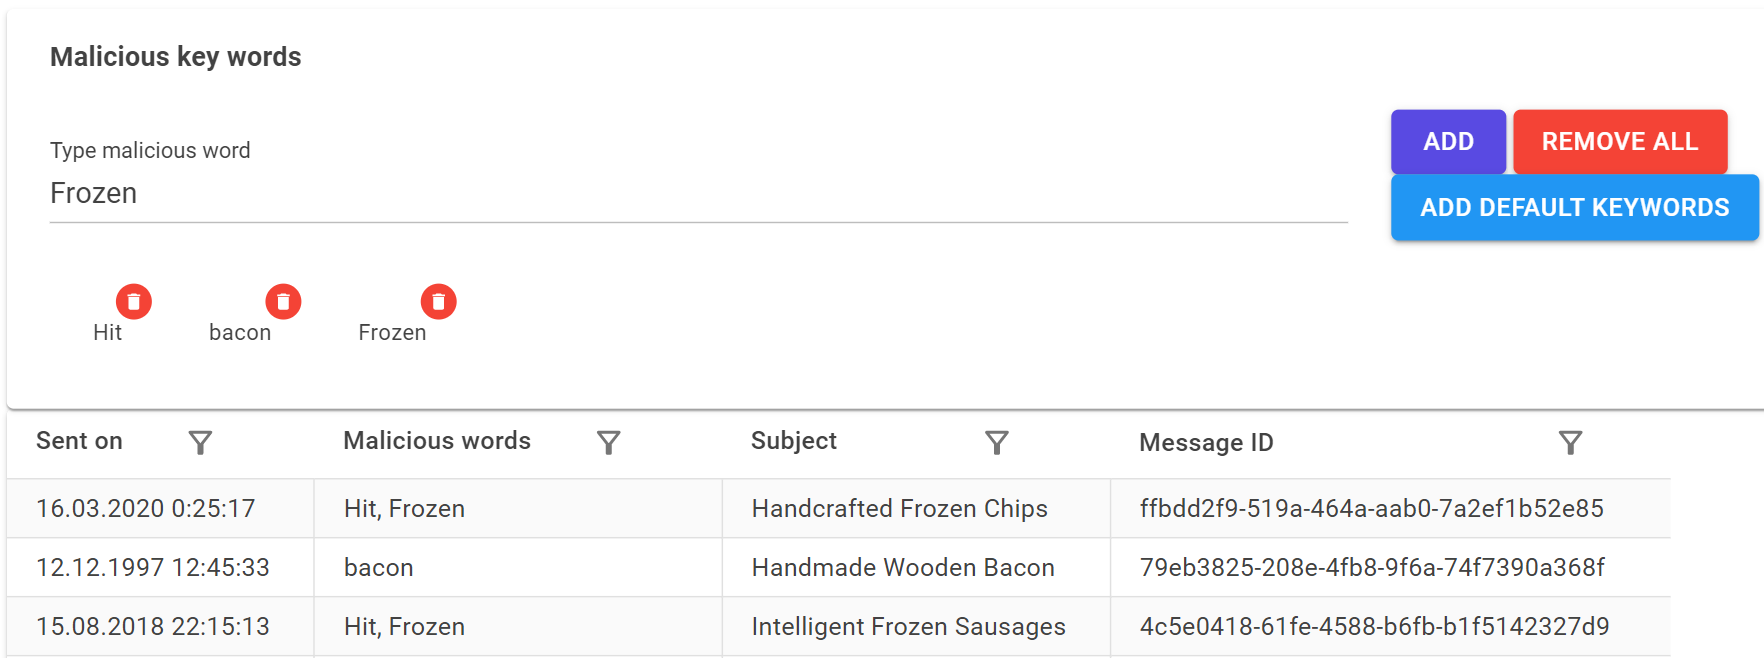
\includegraphics[scale=0.25]{obrazky-figures/Implementace/Blazor/MaliciousWords.png}
            \caption{Graf zobrazující zachycené zprávy v čase, uživatelem vybraných odesílatelů.}
            \label{fig:tableFilterOperators}
        \end{figure}
        
        Další funkcí aplikace je agregování dat pomocí odesílatele. Uživatel může do vyhledávacího pole zadat jméno odesílatele a aplikace mu následně zobrazí veškeré informace o tomto odesílateli, například počet odeslaných zpráv, seznam všech příjemců, seznam všech zaslaných příloh a další relevantní informace.

        Tato funkce umožňuje uživatelům rychle identifikovat informace související s konkrétním odesílatelem a zjistit, jaké zprávy byly odeslány, kdy byly odeslány a komu byly zprávy poslány. To je užitečné zejména v situacích, kdy se vyšetřovatelé snaží rekonstruovat konkrétní události nebo sledovat komunikaci mezi určitými osobami.
    
        \paragraph{Stránky zobrazující detail konkrétní zprávy}        
        Na stránkách, které zobrazují detail konkrétní zprávy, není k dispozici žádná funkčnost. Tyto stránky jsou navrženy jako statické a zobrazují pouze informace o dané zprávě, jako je například datum odeslání, odesílatel, příjemce, předmět a text zprávy.

        Nicméně, abych zajistil co nejlepší \gls{UX}, využil jsem rozšiřujících panelů k zobrazení dodatečných informací. Rozšiřující panely umožňují uživatelům zobrazit další informace o zprávě, které nejsou na první pohled viditelné, jako je text nebo hlavičky emailové zprávy. Rozšiřující panely také pomáhají udržovat stránku čistou a uživatelsky přívětivou.
    
\chapter{Testování}

Testování softwaru je klíčovým procesem v celém vývojovém cyklu, zajišťující kvalitu a spolehlivost výsledného produktu. Cílem testování je zajistit, aby software splňuje definované požadavky. Testování je proces, který by měl být prováděn průběžně během celého vývojového cyklu. K zajištění nejlepších možných výsledků je nutné použít automatizované testy, které lze libovolně spouštět v průběhu vývoje. Je vhodné tyto testy spouštět v pravidelných časových intervalech, aby se případná chyba identifikovala co nejdříve a také byla co nejdříve opravena. Při testování je důležité znát a rozumět případům užití aplikace a otestovat různé možnosti, které by mohl uživatel při používání aplikace vyzkoušet. Testování webové aplikace je provedeno ze dvou důvodů:

\begin{itemize}
    \item Odhalit funkcionální a grafické nedostatky a chyby.
    \item Otestovat \gls{UX} aplikace.
\end{itemize}

V této kapitole popíšu dva druhy testování - testování funkcionality a testování použitelnosti. Na závěr této kapitoly popíšu testování mnou vytvořené aplikace s nezávislým uživatelem. Testování probíhalo tak, že tento uživatel plnil v aplikaci sérií dílčích úloh a já jsem zaznamenával dobu trvání a další hodnoty. Následně zmíním testování aplikace na specifickém případu užití, na kterém jsem testoval i nástroj Xplico a NetworkMiner při získávání znalostí k vytvoření mé aplikace a na závěr vizualizuji případ užití, který demonstruje funkcionalitu aplikace.

\section{Testování funkcionality}
Jedním z nejdůležitějších typů testování je testování funkcionality. Toto testování ověřuje, zda software plní požadavky a specifikace stanovené při návrhu aplikace. Testování funkcionality jsem testoval pouze manuálně. To mi umožnilo ověřit správnost a funkčnost jednotlivých prvků aplikace. Testování jsem prováděl postupně a opakovaně během vývoje a následně po dokončení, abych zajistil, že aplikace bude co nejvíce bezchybná. 

Důraz jsem kladl na ověření správné funkčnosti všech interaktivních prvků aplikace, jako jsou tlačítka, filtrování dat dle data nebo podle identifikátoru relace, pole pro vkládání textu a zobrazených grafů. Konkrétně jsem ověřoval, zda tlačítka reagují a spouští požadovanou reakci, zda aplikace zobrazuje pouze data dle uživatelem zadaných filtrů, zda aplikace správně reaguje na vstupy uživatele a zda jsou všechny interaktivní prvky dostupné a funkční. Dále jsem počítal zobrazené hodnoty v tabulkách, abych ověřil správnost zobrazených grafů. V rámci testování interaktivních prvků jsem se také zaměřil na ověření rychlosti a odezvy aplikace.


Celou aplikaci jsem manuálně otestoval a zkontroloval, že implementovaná funkcionalita funguje. Testování je možné automatizovat automatizovanými testy, které lze vytvářet pomocí nástrojů, jako je například Selenium, Katalon Studio, Cypress. Automatizované testy, lze opakovatelně spouštět a testovat tak aplikaci v pravidelných intervalech.


Během testování jsem identifikoval několik problémů, obzvlášť při zobrazování grafů. Při jejich implementaci se mi stalo, že jsem některá data špatně počítal a zobrazoval tak nepravdivé údaje. Tento problém jsem řešil například při zobrazení všech zachycených zpráv v čase a zobrazoval tak jiný počet zachycených zpráv v daném časovém intervale než ve skutečnosti byl. Tuto chybu, jsem úspěšně vyřešil stejně tak jako ostatní.

\section{Testování použitelnosti}
    Internet se stal součástí každodenního života a lidé používají různé webové aplikace, ať už k práci či zábavě několikrát denně. Z tohoto důvodu je důležité zajistit, aby webové stránky byly uživatelsky přívětivé. Testování použitelnosti je proces při kterém se měří a identifikují slabiny rozhraní webové stránky za účelem zlepšení uživatelské přívětivosti.
    
    Pokud jsou stránky uživatelsky nepřívětivé a uživatel se na stránce neorientuje, může to znamenat nedůvěru v produkt či službu, kterou stránky reprezentují. To může mít za následek, že uživatel opustí stránku a hledaný produkt či službu se pokusí najít jinde. Z tohoto hlediska je uživatelská přívětivost klíčovým faktorem, obzvlášť pro internetové obchody. 
    
    Existují různé techniky jak testovat použitelnost webových stránek. Mezi ty nejpoužívanější patří:
    \begin{itemize}
        \item Analýza úkolů --- proces, při kterém se vytvoří různé úkoly či případy užití, které by uživatel typicky prováděl. Poté se tyto úkoly předají subjektu a analyzují se uživatelem prováděné kroky k jejich dokončení. Tato technika byla použita při testování použitelnosti mnou vytvořené Blazor aplikace.
        \item Sledování chování uživatele --- sledování chování uživatele ze zaměřuje na chování uživatele na stránce, např. průměrná doba stráveného času na stránce, geografické poloze uživatelů, bounce rate\footnote{Bounce rate je ukazatel, který udává procento návštěvníků, kteří opustili webovou stránku po prohlédnutí pouze jedné stránky. Vyšší bounce rate obvykle naznačuje, že uživatelé nenachází na stránce to, co hledají, nebo že je design stránky nedostatečně přehledný.}, atd. Existují nástroje, jenž tato data zaznamenávají automatizovaně. Mezi tyto nástroje patří například Google Analytics nebo Hotjar.
        \item A/B testování --- A/B testování je založeno na kvantitativním testování, vyžaduje dvě či více verzí webových stránek a určitému množství testovacích uživatelů. Testovací uživatelé se rozdělí na skupiny dle počtu verzí webových stránek a následně se zaznamenává uživatelská reakce a použitelnost na každou z verzí.
    \end{itemize}
    
    Každá z těchto technik má silné a slabé stránky a výběr správné závisí na okolnostech a zdrojích. Kombinací uvedených či jiných metod lze dosáhnout lepších výsledků než použitím pouze jedné techniky.

    \section{Testování aplikace}
    V této části popíšu, jak jsem testoval aplikaci se soutěžním příkladem, který byl také použit k otestování nástroje Xplico a NetworkMiner v předešlé kapitole~\ref{sec:XplicoNetworkMiner}. Dále také popíšu jak jsem aplikaci otestoval technikou analýzy úloh, kdy jsem vzal nezávislého uživatele, který neměl s aplikací předešlou zkušenost a analyzoval, jak s aplikací pracuje. Na závěr této sekce uvedu grafický případ užití, který slouží k demonstraci funkcionality aplikace.

    
        \subsection{Specifický případ užití}
        Pro tento případ užití jsem využil stejný specifický případ jako při testování nástroje Xplico a NetworkMiner viz kapitola~\ref{sec:XplicoNetworkMiner}. V tabulce~\ref{tab:PleskalizerSpecialUseCase} je zaznamenáno jak lze jednotlivé úlohy vyřešit pomocí mnou vytvořené Blazor aplikace.
\begin{center}
\begin{table}[ht]
    \centering
    \def\arraystretch{1.5}
    \begin{tabular}{| p{0.02\linewidth} | p{0.93\linewidth} |}
    \hline
        \textbf{1}   & \textbf{Jaká emailová adresa náleží Anně?} \\ \hline
            & Zobrazení kolekce zpráv (\textbf{L7} -> \textbf{SMTP} -> \textbf{Client messages}). U jména Anny lze vidět emailovou adresu a tedy odpověď: \textit{"sneakyg33k@aol.com"} \\ \hline
            
        \textbf{2}   & \textbf{Jaká je emailová adresa milence Anny?} \\ \hline
            & Zobrazení kolekce zpráv (\textbf{L7} -> \textbf{SMTP} -> \textbf{Client messages}). Analyzováním jednotlivých zpráv zaslaných Annou lze určit odpověď: \textit{"mistersecretx@aol.com"} \\ \hline

        \textbf{3}   & \textbf{Jaké dva předměty řekla Anna svému milenci aby přinesl?} \\ \hline
            & Zobrazení kolekce zpráv (\textbf{L7} -> \textbf{SMTP} -> \textbf{Client messages}). Vyhledání zprávy pro adresáta \textit{"mistersecretx@aol.com"}. V detailu zprávy v sekci \textbf{Email} -> \textbf{Payload} lze v obsahu zprávy vyčíst odpověď: \textit{fake passport and a bathing}  \\ \hline

        \textbf{4}   & \textbf{Kolik příloh odeslala Anna celkem?} \\ \hline
            & Zobrazení kolekce zpráv (L7 -> SMTP -> Client messages). Otevřením otevíracího panelu s názvem \textit{"Aggregation"} a napsáním jména Anny do vstupního pole se zobrazí agregovaná data ze všech emailových zpráv, zaslaných Annou včetně počtu příloh. \\ \hline

        \textbf{5}   & \textbf{Název přílohy, kterou Anna poslala svému milenci?} \\ \hline
            & Zobrazení kolekce zpráv (\textbf{L7} -> \textbf{SMTP} -> \textbf{Client messages}). Vyhledání zprávy pro adresáta \textit{"mistersecretx@aol.com"}. V detailu zprávy v sekci \textbf{Email} -> \textbf{Attachments} lze v kolekci příloh zprávy vyčíst odpověď: \textit{"secretrendezvous.docx"} \\ \hline

    \end{tabular}
    \caption{Specifický případ užití mnou vytvořené Blazor aplikace.}
    \label{tab:PleskalizerSpecialUseCase}
\end{table}
\end{center}

        \subsection{Analýza úkolů}
        Při testování technikou analýzy úkolů jsem použil dva případy užití. Případy užití vykonával můj spolužák (dále jen uživatel). Pro uživatele jsem připravil sérii úkolů, které poté vypracoval. Práci dílčích úkolů jsem měřil stopkami a následně jsem zaznamenal, jak se uživateli s aplikací pracuje. Uživatel neměl žádnou předešlou zkušenost s mojí aplikací a při konání jednotlivých úkolů aplikaci viděl poprvé. Při analyzování uživatele vykonávajícího jednotlivé úkony jsem sledoval následující faktory:
        \begin{itemize}
            \item Rychlost, s jakou uživatel plnil úkoly.
            \item Schopnost uživatele najít požadované informace.
            \item Způsob, jakým uživatel interagoval s webovým rozhraním.
        \end{itemize}
        Do následující tabulky~\ref{tab:PleskalizerTesting} jsem zaznamenal výsledky z testování na uživateli. Jednotlivé vlastnosti jsem ohodnotil číslicí 0 až 10 s tím, že číslo 0 znamená zápornou hodnotu a 10 kladnou hodnotu. Jednotlivé úkoly, které uživatel vypracovával:
            \begin{enumerate}
                \item Kolik zachycených komunikací má případ s názvem \textit{"Network puzzle"}

                % L3
                \item Jaký je nepoužívanější protokol na vrstvě L3?

                % L4
                \item Z jaké adresy se odeslalo nejvíce zpráv v zachycené komunikaci na vrstvě L4. Kolik zpráv z této adresy bylo odesláno a na jaké porty?

                % DNS
                \item Kolik je dotazů a kolik odpovědí v DNS komunikaci?
                \item Jaký je nejčastější reply code?
                \item Kolik zpráv je od 6. 2. 1995 do 2. 4. 1999?

                % HTTP Requests
                \item kolik dotazu je na url adresu wikipedia?
                \item jaký je nejčastější typ dotazu?
                \item Kolik příloh typu \textit{.mp4} bylo odesláno při http dotazu?

                % http response
                \item Kolik zpráv mělo odpověď 4xx mezi datem 20. 5. 1987 a 28. 4. 1991?

                % smtp client
                \item Kolik zpráv má uživatel \textit{"Ann Dercover"}?
                \item Co je obsahem zprávy uživatele \textit{"Ann Dercover"} příjemci \textit{"mistersecretx@aol.com"} a kolik zpráva obsahuje příloh
                \item Kdo poslal nejvíce zpráv?
                \item Kolik bylo celkem odesláno příloh a jakého typu bylo nejvíc odesláno?
                \item Obsahuje některá ze zpráv v předmětu nebo obsahu zprávy slovo kokain?
                \item Kolik zpráv odeslal uživatel se jménem \textit{"Zola97"} od roku 2002?
                
            \end{enumerate}
    
    % \begin{landscape} % switch to landscape mode
        \begin{table}[h]
            \centering
            \label{tab:PleskalizerTesting}
            \begin{tabular}{|p{1cm}|p{4cm}|p{1.5cm}|p{3cm}|p{2cm}|p{2.5cm}|p{2cm}|p{2cm}|}
                \hline
                Úkol & Čas na dokončení & Chyby & Snadnost použití (1-10)\\ \hline
                1. & 28s    & 0 & 8     \\ \hline
                2. & 13s    & 0 & 10    \\ \hline
                3. & 1min 14s    & 0 & 8     \\ \hline
                4. & 22s    & 0 & 10    \\ \hline
                5. & 44s    & 0 & 9     \\ \hline
                6. & 1min 41s   & 0 & 10    \\ \hline
                7. & 1min 53s   & 0 & 9     \\ \hline
                8. & 22s    & 0 & 10    \\ \hline
                9. & 33s    & 0 & 9     \\ \hline
                10. & 1min 5s   & 0 & 7     \\ \hline
                11. & 3min 32s  & 0 & 6     \\ \hline
                12. & 1min 3s   & 0 & 7     \\ \hline
                13. & 14s   & 0 & 10    \\ \hline
                14. & 7s    & 0 & 10    \\ \hline
                15. & 2min 16s  & 0 & 6     \\ \hline
                16. & 59s   & 0 & 9     \\ \hline
                
            \end{tabular}
            \caption{Výsledky analýzy použitelnosti.}
        \end{table}    
    % \end{landscape}

    \subsection{Případ užití aplikace}
        Následující diagram užití slouží k vizuální reprezentaci různých scénářů, které lze provádět s tímto nástrojem. Tento diagram zahrnuje všechny funkcionality mnou vytvořeného nástroje k vizualizaci forenzně síťových dat.
        \begin{figure}[H]
            \centering
            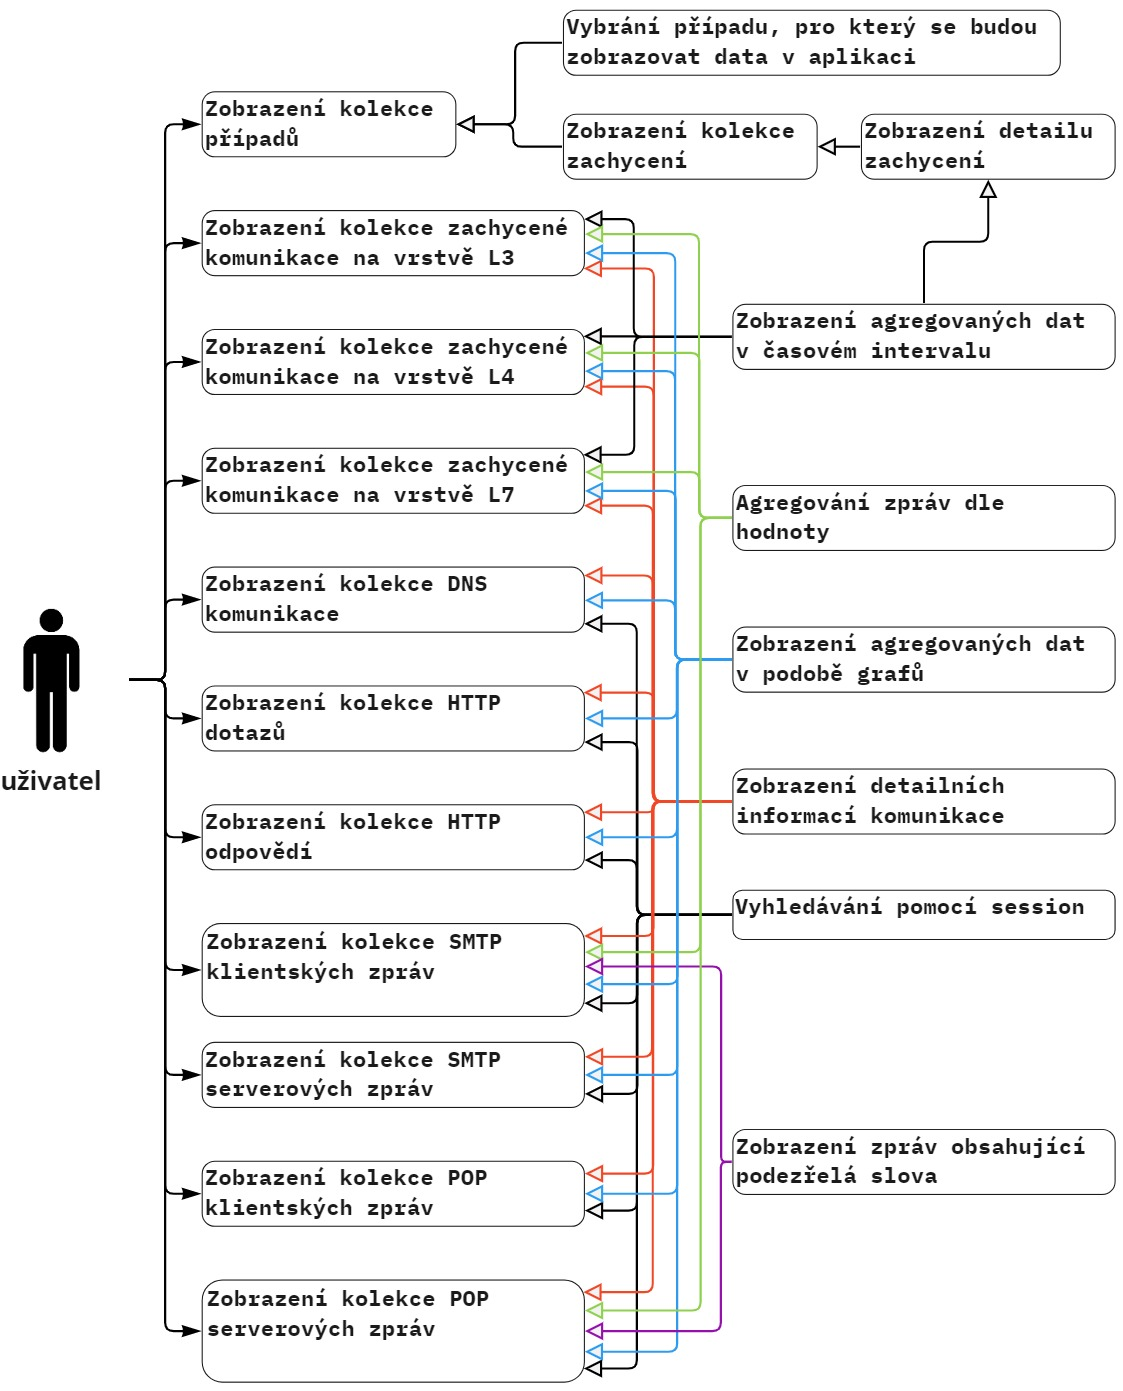
\includegraphics[scale=0.4]{obrazky-figures/usecases/MyApp.jpg}
            \caption{Případ užití, demonstrující funkcionalitu mnou vytvořené Blazor aplikace.}
            \label{fig:PleskalizerUseCase}
        \end{figure}

\chapter{Závěr}

Cílem práce bylo vytvořit uživatelsky přívětivou webovou aplikaci, která bude sloužit vyšetřovatelům jako nástroj k vizualizaci zachycených forenzně síťových dat. Pomocí tohoto nástroje tak budou moct vyšetřovatelé rychleji a efektivněji prošetřovat činy v rozporu se zákonem a identifikovat tak pachatele.

Nejprve bylo nutné si nastudovat forenzní síťovou analýzu jako takovou k porozumění problematiky. Po nastudování potřebných informací jsem analyzoval již existující nástroje. Analyzování těchto nástrojů jsem prováděl přímo v aplikaci, případně ze snímků či videí. Při analýze jsem se zaměřil na \gls{UX} a \gls{UI} nástrojů tak abych poté navrhl aplikaci, která by byla uživatelsky přívětivá a prospěšná v oblasti vizualizace forenzně síťových dat. Důkladnou analýzu jsem provedl u nástroje Xplico a NetworkMiner. U těchto nástrojů jsem vytvořil případ užití demonstrující jejich funkcionalitu a také jsem tyto nástroje podrobil testovacímu případu.

Poté jsem začal s návrhem mé aplikace. Nejprve jsem navrhl definici aplikačního rozhraní, abych definoval jak bude komunikovat webová aplikace se serverem společně s objekty pro datový přenos. Dalším krokem bylo navrhnout uživatelské prostředí. Nejdříve jsem začal vytvářet drátové modely, abych navrhl funkcionalitu a optimální rozvržení komponent na jednotlivých stránkách. Následně jsem začal vytvářet grafické modely, které už měli reprezentovat výsledný vzhled aplikace.

Nedílnou součástí práce byla implementace. Po dokončení všech návrhů jsem začal vytvářet serverovou část, která komunikuje s webovou aplikací a slouží k přenesu dat. Hlavním důvodem tvorby serverové části je otestovaní správné komunikace ze strany webové aplikace. Jelikož hlavním tématem této práce je především webová aplikace vizualizující forenzně síťová data, nevěnoval jsem kvalitě kódu na serverové části tolik pozornosti. Dále bylo potřeba vytvořit data, která by zaplnila aplikaci a bylo možné demonstrovat implementovanou funkcionalitu. Některá data jsem vytvořil ručně abych demonstroval testovací případ použitý při analýze nástroje Xplico a NetworkMiner. Zbylá data jsem vygeneroval pomocí knihovny Bogus. Jakmile byla serverová část funkční a server vracel skrze aplikační rozhraní data, začal jsem vytvářet webovou aplikaci. K tomu jsem použil framework od společnosti Microsoft Blazor, který překládá C\# kód do WebAssembly, které jede ve webovém prohlížeči. Výsledná webová aplikace byla navržena a modularizována tak, aby případná rozšiřitelnost byla jednoduchou záležitostí. Aplikace také byla řádně otestována mnou samotným a také proběhlo testování s uživatelem, který s aplikací neměl předchozí zkušenost. 

\clearpage

\label{sec:forensicsTools}